\documentclass[12pt]{article}
\usepackage[margin = 1in]{geometry}
\usepackage[USenglish]{babel}
\usepackage{natbib}
\usepackage{graphicx}
\usepackage{fancyhdr}
\usepackage{setspace}
\usepackage{amsmath}
\usepackage{lscape}
\usepackage{dcolumn}
\usepackage{xcolor}
\usepackage{subcaption}
\usepackage{enumerate}
\usepackage{longtable}
\usepackage{tabularx}
\usepackage{booktabs}
\usepackage{arydshln}
\usepackage[toc,page,title]{appendix}
\usepackage{titletoc}
\usepackage[colorlinks=true,citecolor=red!50!black,urlcolor=blue!50!black,linkcolor=red!50!black]{hyperref}
\usepackage{chngcntr}
\usepackage{amsthm}

\author{Patrick W. Kraft\footnote{Assistant Professor, University of Wisconsin-Milwaukee, \href{mailto:kraftp@uwm.edu}{kraftp@uwm.edu}.}}

\title{Women Also Know Stuff: \\
%Alternative titles: Let's Talk Politics: A Naive Approach for Measuring Political Sophistication; Talking Politics; Looking for Answers; Why do Women Know Less About Politics? They Don't.
\large{Challenging the Gender Gap in Political Sophistication}\footnote{%Previous versions of this manuscript have been presented at Polmeth 2016, MPSA 2017, EPSA 2017, ISPP 2017, APSA 2017, the Toronto Political Behavior Meeting 2018, and Zurich Text as Data 2019. 
I thank Alexa Bankert, Jason Barabas, Scott Clifford, Andy Delton, Kathy Dolan, Peter DeScioli, Stanley Feldman, Roy Gava, Fabrizio Gilardi, Jennifer Jerit, Yanna Krupnikov, Emmy Lindstam, Hannah Nam, Michael Peress, Daniel Rubenson, R\"udiger Schmitt-Beck, and Arthur Spirling for helpful comments on previous versions of this manuscript. Special thanks to C{\'e}line Colombo, Scott Clifford, and Jennifer Jerit for sharing their data. The manuscript and code are available on GitHub: \url{https://github.com/pwkraft/knowledge}.}
} % Milena Djourelova, Anne Sch\"afer, Timon Forster, Simon Ellerbrock, Christiane Grill, Manuel Neumann, 
\date{}

% sans serif font
\renewcommand{\familydefault}{\sfdefault}

% assumption block
\newtheorem{assumption}{Assumption}

\begin{document}
\maketitle
%\onehalfspacing
\doublespacing
\thispagestyle{empty}

%\begin{center}
%-- WORK IN PROGRESS -- \\
%PLEASE DO NOT CITE OR REDISTRIBUTE WITHOUT PERMISSION
%\end{center} 

\hfill
\begin{abstract}\singlespacing
\noindent This paper proposes a simple but powerful framework to measure political sophistication based on open-ended survey responses. \textit{Discursive sophistication} uses automated text analysis methods to capture the complexity of individual attitude expression. I validate the approach by comparing it to conventional political knowledge metrics in multiple studies using different batteries of open-ended items across four languages. The new measure casts doubt on the oft-cited gender gap in political knowledge: Women might know fewer facts about institutions and elites, but they do not differ substantively in the sophistication of their expressed political attitudes.


\vspace{\baselineskip}
\noindent \textit{Keywords}: political sophistication, gender gap, open-ended responses, text analysis

\vspace{\baselineskip}
%\noindent \textit{Word count}: 5873 (via TeXcount)
\end{abstract}
\hfill

\newpage\setcounter{page}{1}
% REPLACE: "recall" instead of "factual" knowledge questions
% INTRO: motivate process/structure NOT content

% OUTLINE INTRO %
% 1. Assessing political competence is important, but the measurement debate remains unresolved
% 2. Factual knowledge questions are insufficient, we should focus on what people know and not what they don't know
% 3. This is where my measure comes in, describe basic idea and contribution
% 4. Outline of the paper and describe basic findings + conclusion

One of the most important tasks for citizens in modern democracies is to vote for candidates who represent their interests and to hold elected officials accountable. While there have been longstanding debates about whether citizens are sufficiently informed to fulfill this task, fundamental issues regarding the measurement of knowledge continue to plague the discipline \citep{mondak2001developing,sturgis2008experiment,pietryka2013analysis}. Most analyses rely on survey questions that assess individuals' ability to recall basic facts about political institutions and officeholders \citep[e.g.,][]{zaller1990political,carpini1996americans}.\footnote{Others rely on broader conceptualizations of sophistication that incorporate additional dimensions such as education and income \citep[e.g.,][]{jacoby2006value}.} In principle, these quizzes should cover information that is necessary and/or sufficient for citizens to make competent decisions in a given context \citep{lupia2006elitism}. Yet, determining such a set of relevant items proves to be extremely difficult, especially since there are systematic differences in types of knowledge \citep{barabas2014question}. Even within a given policy area, people may disagree about which facts are crucial for political competence due to inherent value differences \citep{lupia2015uninformed}. 

Given these difficulties, empirical studies involving political knowledge and competence usually rely on a set of off-the-shelf recall questions rather than justifying their item selection theoretically. As \citet[219]{lupia2006elitism} points out, ``[m]ost political knowledge questions are not derived from a replicable or transparent logic about how their answers bear on a voter's ability to make decisions of a particular quality.'' It is therefore not surprising that conventional metrics do not properly capture policy-specific information \citep[e.g.,][]{gilens2001political} or other knowledge relevant to citizens' preferences and decision-making \citep[43--68]{graber2001processing}. In a recent review, \citeauthor{cramer2017fact} eloquently summarize: ``All of this work suggests that we are missing a lot by equating information levels as measured in traditional knowledge batteries with civic competence. By focusing on \textit{what people do not know} rather than what they do know and how they use that information, we are likely missing the empirical reality of citizens' political knowledge'' \citeyearpar[756, emphasis added]{cramer2017fact}.
%In other words, rather than trying to examine how people arrive at their preferences, researchers have turned the logic upside down by measuring which facts citizens do not know, irrespective of whether these facts are necessary for competence or not. In an effort to shift the focus from irrelevant facts citizen's don't know to how they arrive at their preferences...

In an effort to shift the focus directly on \textit{what people do know}, I propose a measure of \textit{discursive sophistication} that is based on how people discuss their political preferences in open-ended survey responses. Specifically, I develop a framework to assess whether beliefs and opinions in a given political domain are expressed in a more elaborate manner---a question that is not directly discernible from off-the-shelf factual knowledge items. The approach is therefore \textit{naive} in that it does not presuppose pieces of information as necessary for political competence but rather examines the respondents' justification of their preferences at face value. Measuring sophistication based on how people talk about politics provides two major advantages compared to off-the-shelf factual knowledge items: (1) it captures the extent to which a respondent's political beliefs are based on elaborate reasoning, and (2) it can easily pinpoint competence in specific areas by incorporating targeted open-ended items.

I validate the measure across multiple data sets by comparing it to conventional factual knowledge scores as predictors of various indicators of competence. While the measures share a considerable amount of variance, they are far from equivalent. Indeed, discursive sophistication is a stronger predictor of turnout and other forms of political participation than traditional metrics. After validating the measurement approach, the paper illustrates how discursive sophistication can help refine previous insights in the literature by re-examining an oft-cited finding in empirical research---the gender gap in political knowledge. Contrary to previous research, I find no evidence for such a gap in discursive sophistication. While women might score lower than men on factual knowledge about political institutions and elites, there are no differences in the complexity of expressed political attitudes. This divergence can be explained by the fact that open-ended responses allow women to focus on different issues than men. Altogether, discursive sophistication is shown to be a useful ancillary measure that expands our understanding of political competence and can help improve the development of new factual knowledge questions.



\section*{Attitude Expression and Elaborate Reasoning}
% Style over Substance?
% In-Depth Processing and Attitude Expression

% OUTLINE THEORY %
% 1. Everyone uses knowledge, and it's usually off-the-shelf stuff
% 2. Since it's infeasible to come up with new knowledge battery for every problem, Druckman argues that we should focus on the process rather than the content/substance
% 3. Previous researchers have induced in-depth processing by asking people to justify their preferences
% 4. I ask the question of how people should justify their preferences if they engage in in-depth processing! 
% 5. Examining how people justify their preferences is also important because that's how social infleunce etc. is transmitted.
% 6. (optional) Segway to discuss how these attributes of elaborate processing and sophisticated belief systems should be expressed in open-ended responses.

%In modern democracies, citizens can engage in politics through various means such as voting in local, state, or federal elections. Depending on the institutional setup, they may also directly decide on specific policies through referenda. A common concern in these contexts is whether citizens are able to make high quality decisions in accordance with their underlying interests. Given that

%Rather than trying to develop recall items that presupposes a set of facts as necessary for political competence, I therefore analyze \textit{how} individuals discuss their preferences related to a given political task.

Most studies on political attitudes and public opinion consider individual political knowledge in one way or another---either directly as an outcome variable of interest, as a major explanatory factor, or as an important confounder to control for. In order to measure the underlying latent concept, researchers commonly rely on short batteries of standard recall questions on basic facts about the political system. One canonical article proposing such a battery--\citet{carpini1993measuring}--has been cited approximately 800 times between its publication and the writing of this manuscript. Figure~\ref{fig:carpini} shows the yearly citation count over time; the trend illustrates how political knowledge remains a concept of intense scholarly interest---and that it is frequently measured using standard off-the-shelf recall questions.

\begin{figure}[h]\centering
	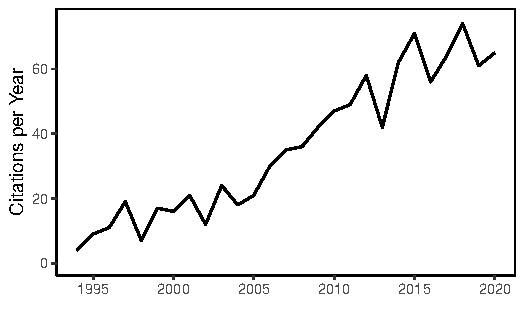
\includegraphics{/data/Dropbox/Uni/Projects/2016/knowledge/fig/cites.pdf}
	\caption[Yearly citation count of \citet{carpini1993measuring}]{Yearly citation count of \citet{carpini1993measuring} based on Google Scholar.}\label{fig:carpini}
\end{figure}

To be fair, it is not always feasible for researchers to develop new sets of knowledge items that specifically target relevant information to make competent decisions in any particular context. Given that there is usually no consensus about what information is necessary in the first place, \citet{druckman2014pathologies} proposes abandoning recall questions as measures of ``quality opinion.'' Instead, the author advocates ``\textit{less} focus on the \textit{content/substance} of opinions [...] and \textit{more} on the \textit{process} and specifically the \textit{motivation} that underlies the formation of those opinions'' \citeyearpar[478, emphasis in the original]{druckman2014pathologies}. The key distinction should therefore be how citizens approach a political issue and whether they are motivated to engage in elaborate reasoning to arrive at their particular decision.
% a useful alternative is to concentrate on whether people are motivated to engage in elaborate reasoning when forming their preferences.

These motivational underpinnings, in turn, have been a subject of lively research in psychology and adjacent fields. In her influential article, \citet{kunda1990case} distinguished between reasoning driven primarily by directional as compared to accuracy goals; people who engage in accuracy-driven reasoning process information more carefully and tend to rely less on biased strategies or cognitive shortcuts. Importantly, experimental evidence suggests that accuracy goals can be activated by telling participants that they have to \textit{justify their beliefs} in front of others \citep{kunda1990case}. There are several notable examples in political science where researchers rely on this strategy to induce in-depth processing by creating the expectation among participants that they have to explain their decisions at some point in the study \citep[e.g.,][]{tetlock1983accountability,redlawsk2002hot,eveland2004effect,bolsen2014influence}.
% also see tetlock1989social

%I argue that we can turn this logic on its head in order to assess the level of elaboration in political reasoning in public opinion surveys. 
I argue that we can extend this logic to assess the degree to which people engage in elaborate reasoning about a political issue by examining \textit{how} they talk about and justify their preferences \citep[see also][]{rosenberg1988structure,rosenberg1988political}. For example, if respondents are motivated and able to engage in in-depth processing to form quality opinions on a specific topic, they should approach it from multiple perspectives and show awareness of arguments for and against certain positions \citep{cappella2002argument}.\footnote{A similar argument is made by \citet{colombo2016justifications} who investigates the competence of Swiss citizens voting in policy referenda. Colombo conceptualizes competence as a voter's ability to justify his or her political decisions, and measures the concept by manually coding open-ended responses to survey questions.} In other words, how people talk about their political preferences provides insights into their underlying motivation to engage in in-depth reasoning and may ultimately allow us to make inferences about their level of sophistication in a specific issue domain.
%Rather than using people's expectation to provide justifications as a manipulation for accuracy motivations, we can therefore directly assess the level of elaboration in political reasoning by examining how people discuss their own views.

There is an additional reason why it is important to consider how people talk about their political preferences when examining citizen competence and sophistication. Political information often reaches citizens indirectly through conversations with coworkers, friends, and family \citep[see][for a recent example]{druckman2018no}. Studies have further shown that political knowledge itself is transmitted through social interactions, especially since people are able to seek out politically competent discussants \citep{huckfeldt2001social,eveland2009political}. Of course, this information diffusion is fundamentally grounded in how people discuss and justify their political beliefs when talking to each other. A survey--especially if it is conducted face to face--could in theory be characterized as such a \textit{formalized} conversation between two individuals (\citealt{sudman1996thinking}; see also \citealt{grice1975logic,grice1978further}). How people discuss their beliefs in open-ended responses can therefore be informative for individual political competence as well as its crucial role in knowledge transmission through social interaction. 


\section*{Conceptualizing Discursive Sophistication}

% OUTLINE MEASUREMENT %
% 1. How can we characterize in-depth processing in open-ended responses? We don't want to look at textual complexity, as other recent research has done.
% 2. It's about the speaker, not the recipient! This is were the literature on belief systems comes in! Theoretical accounts of political sophistication as the basis for elaborate and in-depth political reasoning
% 3. Derive the three dimensions conceptually, connect them to belief system literature -> survey example!
% 4.-6. Now we discuss how we can measure them in open-ended responses

% How can we characterize the level of sophistication in open-ended responses that engage in more in-dpeth processing? This is where the literature on belief systems comes in.
% Next, I will explore specific attributes that allow us to distinguish more or less elaborate reasoning in open-ended responses.
% If we To the extent that people's political sophistication and competence manifests itself in attitude expression 
% Recent studies in political science, for example, used measures based on the readability or comprehensibility to study the sophistication of political communication
% measuring the degree of elaborate reasoning in verbatim attitude expression

Assessing the complexity of written (or spoken) word has been the subject of longstanding research in linguistics and educational sciences, resulting in a multitude of available metrics. Recently, these measures caught the attention of political scientists who study different forms of elite communication. \citet{spirling2016democratization}, for example, uses a standard readability score based on the ratio of words per sentence and syllables per word to study the linguistic complexity of speeches in the British House of Commons over time. More recently, \citet{benoit2017measuring} expanded on previous metrics to develop a measure of comprehensibility that is more applicable in the realm of politics.
% \citet{spirling2016democratization}: The findings reveal that ministers started to use simple language in the parliament after suffrage was expanded in the middle nineteenth century---presumably in an effort to appeal to the enlarged voter base. 

% TODO: Talbot finds this para confusing
These approaches--and especially the development of metrics specifically suited for political text--are particularly useful when studying elite communication. Yet, they share a critical commonality, namely that they focus on the \textit{comprehensibility} as a measure of complexity: sophistication is evaluated based on a recipient's ease to understand the message. Again, while this is certainly a reasonable approach when studying the effects of elite communication, the inference of interest outlined in this paper is markedly different. My focus is to examine verbatim attitude expression to assess the \textit{messenger's} degree of elaborate reasoning. A message's linguistic style is therefore not of central concern so long as it is unrelated to the actual political content.\footnote{In fact, one might be concerned that pure linguistic complexity is ultimately driven by other factors such as a person's general verbosity or linguistic prowess and therefore not a valid measure of political sophistication.} After all, being hard to comprehend does not necessarily imply that someone put a lot of thought into a statement.
% Reading level measures essentially focus on how hard it is to understand the author. This makes sense if we are primarily interested in the messaging aspect, for example when analyzing speeches of political elites. When it comes to individual levels of sophistication, a pure focus on linguistic patterns are less ideal.
% However, while these techniques are certainly useful to examine complexity in messaging by political elites, they may be highly confounded by personal verbosity and linguistic prowess. Instead of assessing linguistic style, we want to target the complexity in the actual content. Rather than measuring how a specific attitude is delivered, we want to focus on the the complexity in what is being said.
% The inference of interest is not how easy it is to understand someone, but rather how much thought went into what has been said. Both are clearly correlated, but they should not be assumed to be equivalent.
% comprehensibility of the text captures more of the linguistic ability independent of the underlying political content.

In contrast, I propose to target the underlying reasoning that gives rise to an utterance by leveraging the content of open-ended responses in conjunction with the survey structure. Consider for example a questionnaire where respondents are prompted to describe their attitudes toward major presidential candidates and their parties in multiple open-ended items. Each question asks for either positive or negative considerations related to one of the parties or candidates. In developing a measure of political sophistication, we are ultimately interested in people's level of elaboration when justifying their preferences in such a set of open-ended responses. So how would a politically sophisticated person who engages in in-depth processing discuss her views compared to a less informed individual?

From a theoretical perspective, political sophistication usually characterizes a particular \textit{structure} of an individual's system of beliefs about politics. For example, \citet{converse1964nature} emphasizes the importance of the level of conceptualization as the main characteristic of sophistication rather than isolated pieces of factual information. Similarly, \citet{tetlock1983cognitive,tetlock1993cognitive} uses the term \textsl{integrative complexity} to describe the degree to which considerations related to an issue are interconnected. \citet{luskin1987measuring} also defines political sophistication based on the structure of individual belief systems, arguing that they can vary on three separate dimensions: (1) their \textsl{size} -- i.e. the number of cognitions, (2) their \textsl{range} -- i.e. the dispersion of cognition over categories, and (3) their \textsl{constraint} -- i.e. the extent to which cognitions are interconnected in a meaningful way. Political sophistication, in turn, is seen as the conjunction of these dimensions: ``A person is politically sophisticated to the extent to which his or her [political belief system] is large, wide-ranging, and highly constrained'' \citep[860]{luskin1987measuring}. A sophisticated open-ended response based on elaborate reasoning should reflect this notion of complex belief systems.\footnote{It should be no surprise that Converse and others examined open-ended responses in their early studies--albeit from a slightly different perspective than the approach outlined here. Importantly, instead of relying on manual coding of open-ended responses, I develop an automated framework that is easily reproducible and can directly be applied to large surveys.}

Consider again the example of multiple open-ended questions regarding candidate and party preferences in a survey. In such a scenario, we can characterize elaborate reasoning by leveraging variation in response patterns on three levels---across questions, between topics mentioned, and within each topic. For each dimension, I make the following assumptions regarding the way sophistication manifests itself in verbatim responses.

First, let us consider response variation across survey items. Individuals who engage in elaborate processing should hold opinions about each political actor or policy they are asked to discuss. Given a set of multiple open-ended probes focusing on different targets of evaluation, sophisticated respondents should be able to express their attitudes towards each question more or less equally.% in terms of both approval or disapproval.

% 1) Distribution between answers
\begin{assumption}[Opinionation]
Sophisticated respondents hold various opinions about political candidates and issues and are therefore able to respond to each query presented in a survey.
\end{assumption}

Next, the level of elaboration should also be related to the content and topics raised by each individual. Respondents who possess a large and wide-ranging belief system should be able to discuss their views from multiple perspectives rather than focusing only on a single consideration.

% 2) Distribution across topics/considerations
\begin{assumption}[Considerations]
Sophisticated respondents evaluate political actors and issues on multiple dimensions and are therefore able to recall a large number of distinct considerations in response to each query presented in a survey. 
\end{assumption}

Lastly, we can examine variation in the way each consideration or topic itself is discussed. Sophisticated respondents should use terms that are highly descriptive of a given topic---for example by mentioning interest rates or unemployment when talking about economic policies.
% rather than broad terms that could be attributed to any topic and are not clearly related to politics.

% 3) Distribution within topics
\begin{assumption}[Word Choice]
Sophisticated respondents use terms that are clearly associated with a specific topic.
\end{assumption}

Discursive sophistication in attitude expression is then defined as the conjunction of these three basic dimensions. Overall, a highly sophisticated individual can be expected to respond to a set of open-ended items by giving a more elaborate response to every question that focuses on multiple considerations using terms that are highly descriptive of each topic. Note that this framework makes no strong assumptions about the type of information necessary to make competent decisions in a given context. Crucially, such a measure of sophistication that is solely based on how individuals discuss their preferences can be directly applied in various settings to target specific political tasks such as choosing between candidates, parties, or policy propositions. Rather than having to devise a new set of questions that attempt to capture information necessary to make competent decisions, we can simply analyze how respondents describe and justify their political preferences in verbatim.
% In the following, I discuss these three different attributes of open-ended survey responses that should be indicative of sophistication in attitude expression in more detail.


%\clearpage
\section*{Overview of Data Sources and Open Ended Items}
% CUTS: This section should start on page 6

In the following, I apply the theoretical framework outlined above to examine discursive sophistication in multiple surveys employing different sets of open-ended questions. Each survey focuses on sophistication in the context of distinct political tasks, namely the evaluation of (1) candidates running for public office, (2) broad issue areas such as health care and gun legislation, and (3) specific legislative policy referenda. The data sets are briefly described below.


\subsection*{2012 \& 2016 American National Election Study}
The main analyses are based on the 2012 and 2016 wave of the American National Election Study (ANES), each of which consists of a representative survey of about 5000 adults in the months before the US Presidential election in each year. About 2000 respondents in both waves participated in face-to-face interviews while the remaining respondents filled out the survey online. For the purpose of the present analyses, I rely on pooled datasets while controlling for differences in survey mode. Discursive sophistication is evaluated using a set of open-ended questions in which respondents were asked to list anything in particular that they like/dislike about the Democratic/Republican party as well as anything that might make them vote/not vote for either of the Presidential candidates. They were probed by the interviewer asking ``anything else?'' until the respondent answered ``no.'' Overall, there are a total number of 8 open-ended responses where individuals described their beliefs and attitudes towards political actors. Individuals who did not respond to all of the open-ended items (420 in 2012; 204 in 2016), or who responded in Spanish (228 in 2012; 43 in 2016), are excluded from the analysis.


\subsection*{2015 YouGov Survey}
In order to replicate and extend the main analyses, I rely on a separate nationally representative survey employing an alternative set of open-ended responses. The data was collected by YouGov in December 2015 and contains responses of 1000 U.S. citizens.\footnote{See \citet{clifford2018disgust} for details on the study.} As part of this study, respondents were asked to describe their attitudes towards two prominent political issues that were discussed frequently in the media. First, they were asked in a closed format whether they favor or oppose stricter gun laws. Subsequently, they were asked to respond to the following two questions:
\begin{itemize}\setlength\itemsep{0em}
\item Still thinking about the question you just answered, what thoughts came to mind while you were answering that question? Please try to list everything that came to mind.
\item Thinking about the mass shootings that have occurred in the U.S. in the last few years, what factors do you think are responsible for the shootings?
\end{itemize}
Second, the respondents reported on their attitudes towards the Affordable Care Act in a closed format and were then asked to elaborate in their own words by answering the following questions:
\begin{itemize}\setlength\itemsep{0em}
\item Still thinking about the question you just answered, what thoughts came to mind while you were answering that question? Please try to list everything that came to mind.
\item For decades, experts have observed that the United States spends far more per person on health care than any other country. However, the U.S. falls behind on most measures of health care outcomes, such as life expectancy. What factors do you think are responsible for the state of our health care system?
\end{itemize}
Here, discursive sophistication is evaluated based on the verbatim responses to the four preceding questions using the same procedures described above. Compared to the open-ended likes/dislikes items included in the 2012 and 2016 ANES, the questions directly address considerations related to specific policy issues that were prominent in the political discourse at the time of the survey. Respondents who did not provide an answer to any of the open-ended questions were removed from the analysis (48).


\subsection*{Swiss Referendum Survey}
Lastly, I examine survey data on Swiss citizens justifying their vote choices on multiple referenda used in a recent analysis by \citet{colombo2016justifications}. The author compiled a data set of cross-sectional surveys administered in Switzerland after national popular votes on multiple policy propositions. The original surveys were conducted as representative samples after each of thirty-four national policy votes that were held between 2008 and 2012 resulting in a total of about 27,000 observations. However, respondents were only asked to justify their decision for or against a given proposition in verbatim if they participated in the vote in the first place. As such, about 5,000 individuals in the data set did not provide an open-ended response. The remaining respondents were asked to describe the main reason as well as additional justifications for their decision in two separate items. As before, discursive sophistication is evaluated based on verbatim responses to both questions.
% QUESTION wording for Swiss study?



\section*{A First Look at Discursive Sophistication}

%Discursive sophistication is conceptualized based on three levels of variation in a set of open-ended responses.
In order to measure discursive sophistication in these different context, we need to quantify the individual-level variation on each of the three dimensions outlined above. First, when looking at response patterns across questions, high levels of elaboration should display a greater level of \textit{opinionation}, which is based on the degree to which individuals are able to respond to each query presented in a survey more or less equally. We can conceptualize this diversity in relative lengths for each open-ended response as the Shannon entropy across survey items.
\begin{equation}
\text{opinionation}_i = \dfrac{-\sum_{j=1}^J p_{ij} \ln p_{ij}}{\ln J}
\end{equation}
where $p_{ij}$ is the proportion of words in the response of individual $i$ to question $j\in \{1,...,J\}$ relative to the overall size of the individuals' response. The variable ranges from 0 (only one question was answered) to 1 (all questions were answered with the same word length per answer).

Second, we need to quantify the number of \textit{considerations} discussed by each individual. I rely on the structural topic model framework \citep{roberts2014structural} to extract the number of topics mentioned by each respondent in a survey.\footnote{See below for more information on the set of open-ended responses, pre-processing choices, as well as on the topic model specification.} Denote $\mathcal{W}_i$ as the set of words contained in a response of individual $i$. Each word $w\in\mathcal{W}_i$ is assigned to a topic $t^* \in \{1,...,T\} $, such that $P(t^*|w,X_i) > P(t|w,X_i) \forall t\neq t^*$.\footnote{Note that $P(t|w,X_i)=\dfrac{P(w|t)P(t|X_i)}{P(w|X_i)}$. In the context of structural topic models, $X_i$ denotes the covariates used to predict individual topic prevalence \citep[see][for details]{roberts2014structural}.} In other words, each unique term in a response is assigned to the topic that has the highest likelihood of having generated that term, given the model. The set of topics that are mentioned by respondent $i$ across all words in $\mathcal{W}_i$ can then be described as $\mathcal{T}^*_i$ and the number of considerations can be written as:
\begin{equation}
\text{considerations}_i = \dfrac{|\mathcal{T}^*_i|}{\max|\mathcal{T}^*_i|}.
\end{equation}
The measure is re-scaled to range from zero to one by dividing raw count of topics by the maximum number of topics observed across individuals.

%There's a connection between the Benoit Google Scholar argument and the word choice measure, although with opposite conclusions...

The last sophistication component discussed above concerns the way individuals talk about each consideration.

Highly descriptive word choice is conceptualized as the sum of term likelihoods $P(w|t^*)$ given topic assignments over the entire set of words in $\mathcal{W}_i$:
\begin{equation}
\text{word choice}_i = \dfrac{\sum_{\mathcal{W}_i} P(w|t^*)}{\max\left[\sum_{\mathcal{W}_i} P(w|t^*)\right]}
\end{equation}
Again, the measure is re-scaled to range from zero to one by dividing all values by the empirical maximum observed across all individuals in the data.

% TODO: think of new label for opinionation



% TODO: mention factor analysis here, maybe add in appendix

Together, the three measures form a composite metric of sophistication in political attitude expression by calculating their respective average for each respondent. Like each individual component, the resulting \textit{discursive sophistication} score ranges from 0 to 1:
\begin{equation}
\text{discursive sophistication}_i = \tfrac{1}{3}(\text{considerations}_i + \text{word choice}_i + \text{opinionation}_i).
\end{equation}

\footnote{See Appendix~\ref{app:oeinfo} for descriptive information on open-ended responses in each dataset, structural topic model results, and individual components of discursive sophistication. Appendix~\ref{app:topicmodel} contains further details on pre-processing steps and modeling choices for the structural topic models as well as robustness checks, which include preText analyses proposed by \citet{denny2018text}. Lastly, Appendix~\ref{app:variables} provides information on the remaining variables included in the analyses.}

%%%%%%%%%%%%%%%%%%%%%%%%%%%

Before turning to the validation, I begin by directly comparing discursive sophistication to alternative metrics of political knowledge in the 2012 and 2016 ANES. The standard approach to measuring political knowledge in surveys is to ask a set of factual questions about political institutions. The ANES surveys include such a basic item battery, inquiring for example about the number of times an individual can be elected President of the United States, or how the current U.S. federal budget deficit compares to the deficit in the 1990s. I combine responses on these items to form an additive index of \textit{factual knowledge} about politics. As an additional benchmark, I consider \textit{interviewer assessments} of each respondent's political sophistication (see \citealt{bartels2005homer} for an example of a study that relies on interviewer assessments; but cf. \citealt{ryan2011accuracy}).\footnote{Interviewer assessments were only recorded in the face-to-face sample of the ANES.}

\begin{figure*}[h]
    \centering
    \begin{subfigure}[t]{0.5\textwidth}
        \centering
        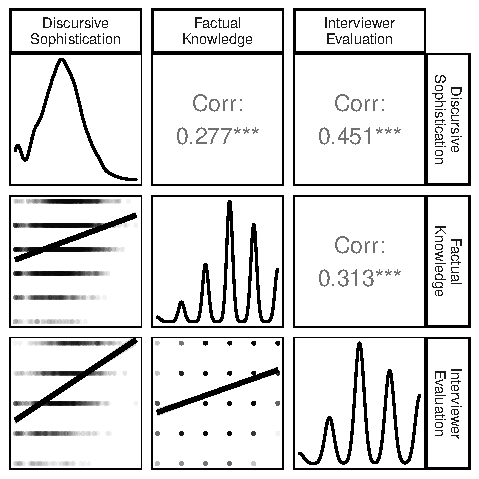
\includegraphics{/data/Dropbox/Uni/Projects/2016/knowledge/fig/anes2012_corplot.pdf}
        \caption{2012 ANES}
    \end{subfigure}%
    ~ 
    \begin{subfigure}[t]{0.5\textwidth}
        \centering
        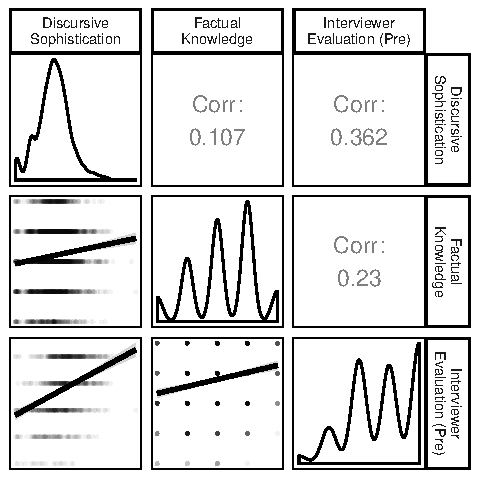
\includegraphics{/data/Dropbox/Uni/Projects/2016/knowledge/fig/anes2016_corplot.pdf}
        \caption{2016 ANES}
    \end{subfigure}
    \caption[Correlation matrix of discursive sophistication and conventional political knowledge metrics]{Correlation matrix of discursive sophistication and conventional political knowledge metrics. The plots on the diagonal display univariate densities for each variable. The panels in the lower triangular display the scatter plot of two measures as well as a linear fit. The upper triangular displays the correlation coefficient. All correlations reported are statistically significant with $p<.05$.}\label{fig:corplot}
\end{figure*}

Figure~\ref{fig:corplot} compares discursive sophistication to the conventional knowledge metrics for both surveys. Each figure presents scatterplots between individual measures (lower triangular), univariate densities (diagonal), and correlation coefficients (upper triangular). The measure of discursive sophistication is positively correlated with both conventional metrics while capturing some additional variation. Interestingly, there is a stronger correlation between discursive sophistication and interviewer evaluations than between factual knowledge and interviewer evaluations ($r=.45$ vs. $r=.31$ in 2012, and $r=.36$ vs. $r=.23$ in 2016). The open-ended measure therefore captures characteristics that influence subjective assessments of sophistication. Interviewers certainly form their impressions throughout the entire survey, but a respondent's verbatim answers seems to be more influential for subsequent knowledge assessments than a respondent's performance on the factual knowledge questions.

Overall, while discursive sophistication and the alternative measures are clearly correlated, the relationship between each metric is far from perfect. To provide some intuition as to whether the variation in discursive sophistication is theoretically meaningful, I present an example of open-ended responses of two individuals in the 2016 ANES who identified as Republicans and scored equally on the factual knowledge score (3 out of 4 correct responses), but varied highly in discursive sophistication. The results are presented in Table~\ref{tab:ex1}.

\begin{table}[ht]\footnotesize\centering
\begin{tabular}{l|p{6.3cm}|p{6.3cm}}
\toprule
	& A: Low Sophistication Response & B: High Sophistication Response \\ \midrule
Clinton (+)		& 																& Politician. \\\hdashline
Clinton (-)		& The fact that she has links to Al-Qaeda. 						& Caught in lies. \\\hdashline
Trump (+)		& 																& Says what he thinks. \\\hdashline
Trump (-)		& He is going to start a civil war. I feel like he is racist. 	& Reality TV star, poor businessman \\\hdashline
Democrats (+)	& 																& Middle class minded. \\\hdashline
Democrats (-)	& 																& Too many handouts. \\\hdashline
Republicans (+)	& 																& Economic growth conscious. \\\hdashline
Republicans (-)	& 																& For the big business. \\\midrule
Disc. Soph. 	& 0.162 														& 0.461 \\\bottomrule
 \end{tabular}
\caption[Example of open-ended responses for low and high scores on discursive sophistication]{Example of open-ended responses for low and high scores on discursive sophistication with equal factual knowledge scores (3 out of 4 correct responses). Column A displays the verbatim responses of an individual who scored low on discursive sophistication and column B displays the verbatim responses of an individual who scored high on the open-ended measure. Each row represents one of the likes/dislikes items included in the analysis. Note that the responses in this table were slightly redacted for readability (spelling errors removed, etc.).}\label{tab:ex1}
\end{table}

Each row in the table represents one of the open-ended responses (like/dislike for each candidate/party). Column A displays the responses of an individual who scored low on discursive sophistication and column B displays the responses of a high scoring individual. Cells are empty if a respondent refused to provide a response. Even though both individuals are measured to have equal factual political knowledge, there are systematic differences in their response behavior that can be attributed to their political sophistication. Overall, respondent A provided a less elaborate response, only focused on a narrow range of issues, and only reported attitudes on two items. Irrespective of whether one agrees with the specific statements or whether they are factually accurate (e.g., Clinton's connection to Al-Qaeda), A's response pattern is suggestive of a less sophisticated political belief system and a lower level of motivation to engage in in-depth reasoning about both parties and candidates. Overall, this initial result suggests that the variation in discursive sophistication captures meaningful differences in response behavior that overlaps with traditional knowledge metrics while displaying some unique variation. The following sections will show that this variation is also politically consequential.



\section*{Discursive Sophistication and Political Competence}

I validate the measure of discursive sophistication by directly examining its effects on individual competences to perform political tasks in modern democracies \citep[cf.][]{lupia2006elitism,lupia2015uninformed}. More specifically, I consider the potential role of political sophistication in promoting (1) engagement and participation in politics, (2) the ability to incorporate new information, and (3) well-justified policy preferences. In the following, each point will be addressed using one of the three data sets described above.
% (5) vote choices that are consistent with underlying interests


\subsection*{Engagement and Participation in Politics}
Political sophistication is often argued to promote individual engagement and participation in politics. In fact, factual knowledge items have been validated in the past based on their strong relationship with outcomes such as turnout and other forms of participation \citep[230--233]{lupia2015uninformed}. Figure~\ref{fig:knoweff} compares the effects of discursive sophistication and factual knowledge in the 2012 and 2016 ANES on four dependent variables related to political engagement: turnout, non-conventional participation, internal efficacy, and external efficacy. The model predicting turnout is estimated via logistic regression while the estimates for the three remaining dependent variables are based on OLS. Each model equation includes both sophistication measures while controlling for gender, education, income, age, race, church attendance, survey mode (face-to-face vs. online), as well as the Wordsum vocabulary score measuring verbal intelligence.

\begin{figure}[h]\centering
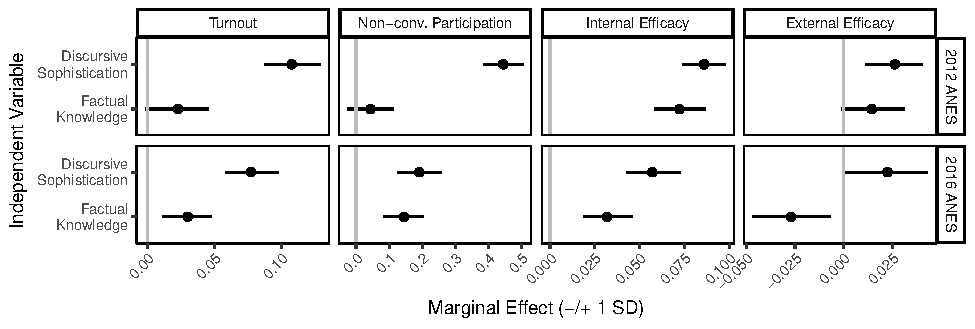
\includegraphics{/data/Dropbox/Uni/Projects/2016/knowledge/fig/knoweff_pres.pdf}
\caption[Effects of sophistication on turnout, non-conventional participation, internal efficacy, and external efficacy in the 2012 and 2016 ANES]{Effects of sophistication on turnout, non-conventional participation, internal efficacy, and external efficacy in the 2012 and 2016 ANES. For each dependent variable, the figure displays the change in expected values after increasing each sophistication measure from -1 to +1 standard deviation from its mean (including 95\% confidence intervals). Model estimates are based on logistic regression (turnout) or OLS (non-conventional participation, internal efficacy, external efficacy). Both sophistication measures are included simultaneously while controlling for gender, education, income, age, race, church attendance, survey mode, and Wordsum vocabulary scores. Full model results are displayed in the appendix, Tables~\ref{tab:knoweff2012} and \ref{tab:knoweff2016}.}\label{fig:knoweff}
\end{figure}

Each panel displays the expected difference in the respective dependent variable for a two standard deviation increase in each sophistication measure, while holding all other variables constant at their means. Overall, discursive sophistication is a stronger predictor of turnout, non-conventional participation, as well as (to a lesser extent) internal and external efficacy. In the 2012 ANES, the positive effect of factual knowledge on participation is statistically indistinguishable from zero when controlling for discursive sophistication. Furthermore, there is a negative effect of factual knowledge on external efficacy in the 2016 ANES. In contrast, the positive effect of discursive sophistication on external efficacy is more consistent with previous research. Considering these initial results, a potential concern may be that discursive sophistication is confounded by personality characteristics that influence verbatim response patterns as well as engagement. Appendix~\ref{app:personality} provides additional analyses controlling for such factors that might drive verbosity (extraversion and being reserved) as well as individual response length itself. The substantive conclusions remain unchanged.


\subsection*{Incorporation of New Information}
Competent citizens should not only engage in politics but are also expected to be sufficiently informed about the issues of the day. As such, they have to be attentive to their media environments and incorporate potentially relevant new information about parties, office-holders, and policies. Indeed, \citet{zaller1990political,zaller1992nature} and others argue that tests of factual information about politics are the best available proxy for awareness. In this analysis I draw on the 2015 YouGov study to explore whether discursive sophistication or factual knowledge serves as a better predictor of people's ability to incorporate new information from media sources. As part of the survey, respondents were asked to read a newspaper article about a fictional infectious disease and were subsequently asked to answer questions about information provided in the article (e.g. regarding symptoms, modes of contraction etc.). I compute an additive index counting the pieces of information that were correctly recalled (\textit{information retrieval}) as a measure of the ability to retrieve information from a news article on a non-partisan issue that is related to public health policies. 

\begin{figure}[h]\centering
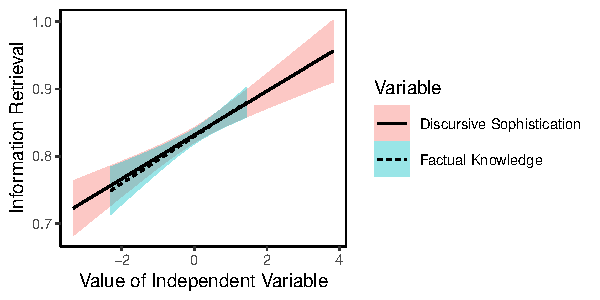
\includegraphics{/data/Dropbox/Uni/Projects/2016/knowledge/fig/yg_disease.pdf}
\caption[Expected information retrieval in the 2015 YouGov Study as a function of political sophistication]{Expected information retrieval in the 2015 YouGov Study as a function of political sophistication (including 95\% confidence intervals). Estimates are based on a linear regression model controlling for education, income, age, church attendance, gender, and race. Full model results are displayed in the appendix, Table~\ref{tab:yg_disease}.}\label{fig:yg_disease}
\end{figure}

Figure~\ref{fig:yg_disease} displays the relationship between political sophistication and disease information retrieval in the 2015 YouGov study. Estimates are based on a linear regression model controlling for education, income, age, church attendance, gender, and race. As a benchmark for discursive sophistication, I again consider the effect of factual knowledge based on a battery of eight items similar to the knowledge questions in the ANES. Both discursive sophistication as well as factual knowledge increase the amount of information individuals are able to recall from a news article discussing a fictional disease. Similar to the previous results, the effects are stronger for discursive sophistication than for factual knowledge scores. The degree to which citizens discuss their own political beliefs in a more elaborate manner is not only a stronger predictor of political engagement but also serves as a better proxy for the ability to incorporate new information about a non-partisan issue.


\subsection*{Well-Justified Policy Preferences}
Beyond the ability of incorporating new information, competent citizens should be knowledgeable about the underlying policies themselves and be able to justify their own preferences. Here, I explore the extent to which high levels of discursive sophistication correspond to well-justified policy preferences in open-ended responses. As mentioned above, the Swiss surveys included items that asked respondents to explain why they voted in favor or against a given proposition in multiple policy referenda. To corroborate the face validity of discursive sophistication, I examine whether the measure is related to Colombo's \citeyearpar{colombo2016justifications} manual coding of the respondents' \textit{level of justification}, which assessed the content, elaboration, and complexity of open-ended responses.

The results are presented in Figure~\ref{fig:swiss_ggridges}. Since the Swiss post-referendum surveys were conducted in three different languages (German, French, and Italian), I computed the measure of discursive sophistication separately for each group of respondents. The figure displays the distribution of discursive sophistication for each level of justification coded by \citet{colombo2016justifications} as well as the correlation coefficients for both respective variables. Across all three language groups, discursive sophistication is systematically higher among respondents with the highest level of justification and both measures are positively correlated ($r=0.29, 0.25$, and $0.35$, respectively). The proposed measure of discursive sophistication therefore shows a high degree of correspondence with individual levels of justification assessed by independent manual coders.

\begin{figure}[h]\centering
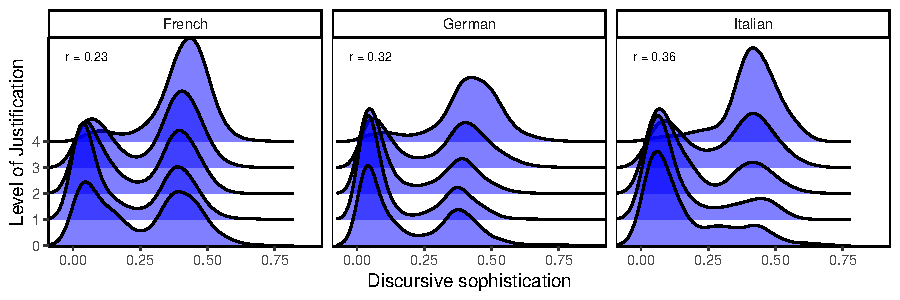
\includegraphics[scale=1]{/data/Dropbox/Uni/Projects/2016/knowledge/fig/swiss_ggridges.pdf}
\caption[Discursive sophistication and manually coded level of justification in Swiss post-referendum surveys]{Discursive sophistication and manually coded level of justification \citep{colombo2016justifications} in Swiss post-referendum surveys. The plot compares kernel densities of discursive sophistication for each manually coded level of justification.}\label{fig:swiss_ggridges}
\end{figure}

To summarize, the results presented thus far indicate that discursive sophistication shares common characteristics with factual political knowledge measures. Compared to conventional metrics, the proposed measure performs as least as well as a predictor of essential competences that allow citizens to engage successfully in politics. In fact, discursive sophistication is a stronger predictor of certain outcomes (such as different forms of political participation) than conventional knowledge scores. In the following, I turn to an application to illustrate how discursive sophistication can help refine important previous insights from the literature on political knowledge.

\clearpage
\section*{Application: The Gender Gap in Political Knowledge}

A common finding in public opinion research is the fact that women have lower levels of observed political knowledge than men. For example, \citet{verba1997knowing} report that women score lower on political information, interest, and efficacy, which decreases their respective levels of political participation. Since gender differences in political information and interest can only partly be explained by resource-related factors such as individual levels of education, the authors diagnose a ``genuine difference in the taste for politics'' between men and women, which they suspect to be driven largely by socialization \citep[see also][]{wolak2011roots}. Indeed, \citet[117]{dow2009gender} describes the systematic gender differences in knowledge ``one of the most robust findings in the study of political behavior.''

The discussion revolving around this apparent gender gap is closely intertwined with the methodological debate about measuring political knowledge. For example, \citet{mondak2004knowledge} suggest that women are more likely to report that they do not know the answer to a recall question whereas men are more inclined to guess. Correcting for the systematic differences in the propensity to guess, however, mitigates the gender gap in knowledge but does not eliminate it completely \citep[see also][]{lizotte2009explaining}. Other aspects of the survey context have been shown to affect gender differences in political knowledge. For example, \citet{mcglone2006stereotype} present evidence that the gender gap is exacerbated in an environment that induces stereotype threat, for example if women are aware of the fact that the study focuses on gender differences or if they are interviewed by a male interviewer. However, gender differences are not only induced by \textit{how} researchers ask their questions, but also by the question \textit{content} itself. For example, \citet{dolan2011women} argues that the gap can be closed by focusing on gender-relevant political knowledge items such as information about women's representation in the federal government \citep[see also][]{graber2001processing,fraile2014does,jerit2017revisiting}. Similarly, \citet{stolle2010women} report that the gender gap disappears when people are asked about more practical issues related to the government (e.g., benefits and services).

Overall, the gender gap has been shown to be influenced by how we ask for political information in surveys, as well as the kind of knowledge that is required for a correct response. Indeed, a comprehensive cross-national analysis of election studies in 47 countries between 1996 and 2011 suggests that question format and content account for large portions of the variance of gender disparities in political knowledge \citep{fortin2016cross}.


\subsection*{Descriptive Results}
How do men and women compare on the different metrics of political sophistication in the surveys analyzed in the present study? Figure~\ref{fig:meandiff} displays the average levels of discursive sophistication as well as conventional metrics comparing both genders. While we observe a sizable and statistically significant gender gap for factual knowledge in both ANES surveys, this difference disappears for discursive sophistication. These results are replicated in the 2015 YouGov survey. As before, we observe a significant gender gap in factual knowledge which disappears using the discursive measure. Of course, it is important to ask whether this absence of a gender gap in discursive sophistication is theoretically meaningful or rather an artifact of the measurement approach itself. 

One way to investigate this question is to explore gender differences in discursive sophistication using the \citet{colombo2016justifications} data and comparing them to her manually coded measure. That way, we can not only examine whether the lack of a gender gap in discursive sophistication replicates using an additional survey, but also check whether there is an equivalent lack of gender differences in Colombo's alternative measure of citizen competence in direct democracies. If discursive sophistication captures a person's motivation to undertake in-depth reasoning and form quality opinions (and assuming these characteristics do not differ by gender), there should be no difference between men and women on either metric (discursive sophistication and Colombo's measure).  As shown in the bottom row of Figure~\ref{fig:meandiff} there are indeed no significant gender differences on \textit{both} metrics across all three languages in the Swiss referendum surveys. The absence of a gender gap is consistent whether open-ended responses are coded manually or using the proposed measure of discursive sophistication.

\begin{figure}[h]\centering
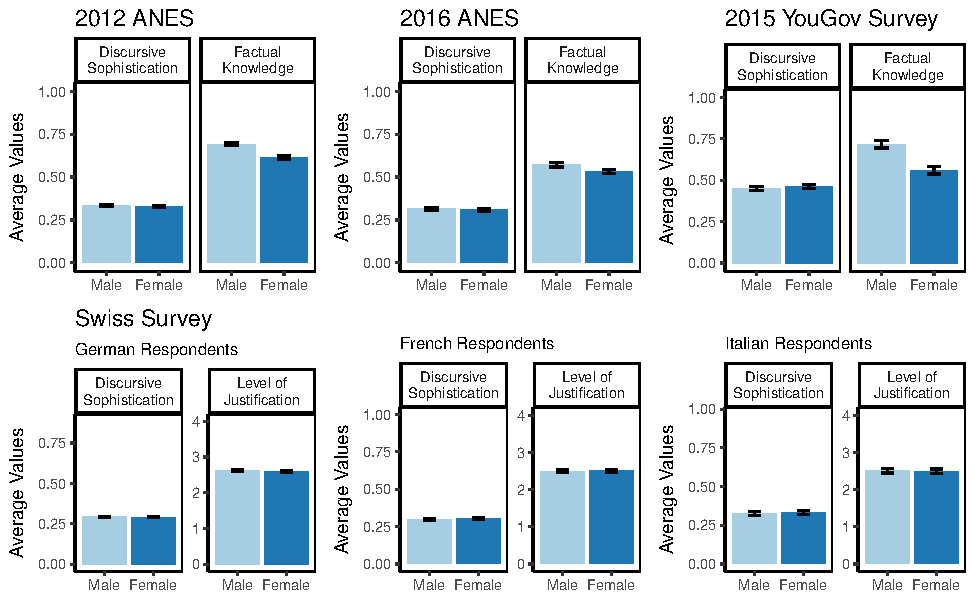
\includegraphics{/data/Dropbox/Uni/Projects/2016/knowledge/fig/meandiff.pdf}
\caption[The gender gap in political sophistication]{The gender gap in political sophistication. The figures display mean levels of sophistication for each measure comparing men and women (including 95\% confidence intervals). Gender differences in factual knowledge in the 2012/2016 ANES and 2015 YouGov survey (top row) are statistically significant with $p<.05$. Gender differences in discursive sophistication and manually coded levels of justification \citep{colombo2016justifications} are not statistically significant.}\label{fig:meandiff}
\end{figure}


\subsection*{Controlling for Alternative Explanations}
Prior research suggests that at least part of the gender gap in political knowledge can be attributed to real discrepancies in resources and engagement. To the extent that differences between men and women can be explained by these underlying factors, they are less likely to be an artifact of the measurement of knowledge itself. Accordingly, we need to control for determinants of political knowledge to provide a more comprehensive examination of the veracity of observed gender differences. Figure~\ref{fig:determinants} displays estimated effects of various potential common determinants of factual knowledge and discursive sophistication on both measures. Previous studies consistently showed that political information levels are positively related to high media exposure, frequent political discussions, education, and income. Furthermore, I include age, race, church attendance, and survey mode (face-to-face vs. online) as additional control variables.

\begin{figure}[h]\centering
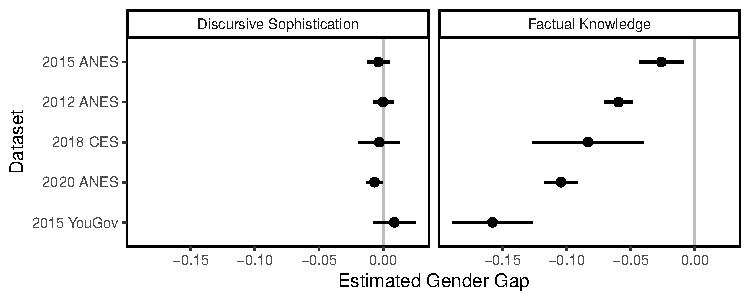
\includegraphics{/data/Dropbox/Uni/Projects/2016/knowledge/fig/determinants.pdf}
\caption[Common determinants of political sophistication]{Common determinants of political sophistication. Estimates are OLS regression coefficients with 95\% confidence intervals. Dependent variables are discursive sophistication as well as factual political knowledge. Full model results are displayed in the appendix, Tables~\ref{tab:determinants_anes} and \ref{tab:determinants_yg}.}\label{fig:determinants}
\end{figure}

After controlling for common determinants, discursive sophistication again reveals no significant differences between men and women in both ANES surveys as well as the 2015 YouGov study. The gender gap in factual political knowledge, however, persists and is substantively as well as statistically significant after controlling for various resource-related factors. Even though women do not perform as well as men on political quizzes, they do not differ substantially in complexity and sophistication when they describe their political preferences. The effects of the remaining variables are quite similar across both measures and different surveys. Knowledge and sophistication is significantly higher among respondents who are more exposed to political news media, discuss politics frequently, are more educated, and have higher income.\footnote{An interesting deviation, however, is the effect of survey mode in the 2012 and 2016 ANES. Respondents in online surveys score significantly higher on factual knowledge than in face-to-face interviews. This difference can be attributed to the fact that individuals are able to look up answers for factual knowledge questions while taking an online survey \citep[cf.][]{clifford2016cheating}. For discursive sophistication, on the other hand, individuals perform better in the face-to-face survey. Open-ended answers in online surveys may be less elaborate because respondents have to manually type their responses.} Overall, the finding that determinants of political sophistication are consistent across models lends additional validity to the open-ended measure.

To summarize, we only observe a significant gender gap when looking at conventional recall-based measures, a result that previous research (at least partly) attributed to the content (i.e., focusing on issues that are less relevant to women) and format (i.e., stereotype-threat and guessing) of the question batteries. When using the alternative measure---discursive sophistication---any evidence for systematic differences between men and women disappears.


\subsection*{Explaining the (Lack of the) Gender Gap}
If it is the case that women are able to close the gender gap in discursive sophistication because they are able to focus on different considerations that are salient to them when discussing their political preferences, we should observe systematic variation in the issues men and women discuss in open-ended responses. Based on the structural topic model used to compute discursive sophistication, I now examine the subset of topics that showed the largest absolute gender difference in topic prevalence in the 2012 and 2016 ANES. The results are displayed in Figure~\ref{fig:stm_gender}.

\begin{figure}[h]\centering
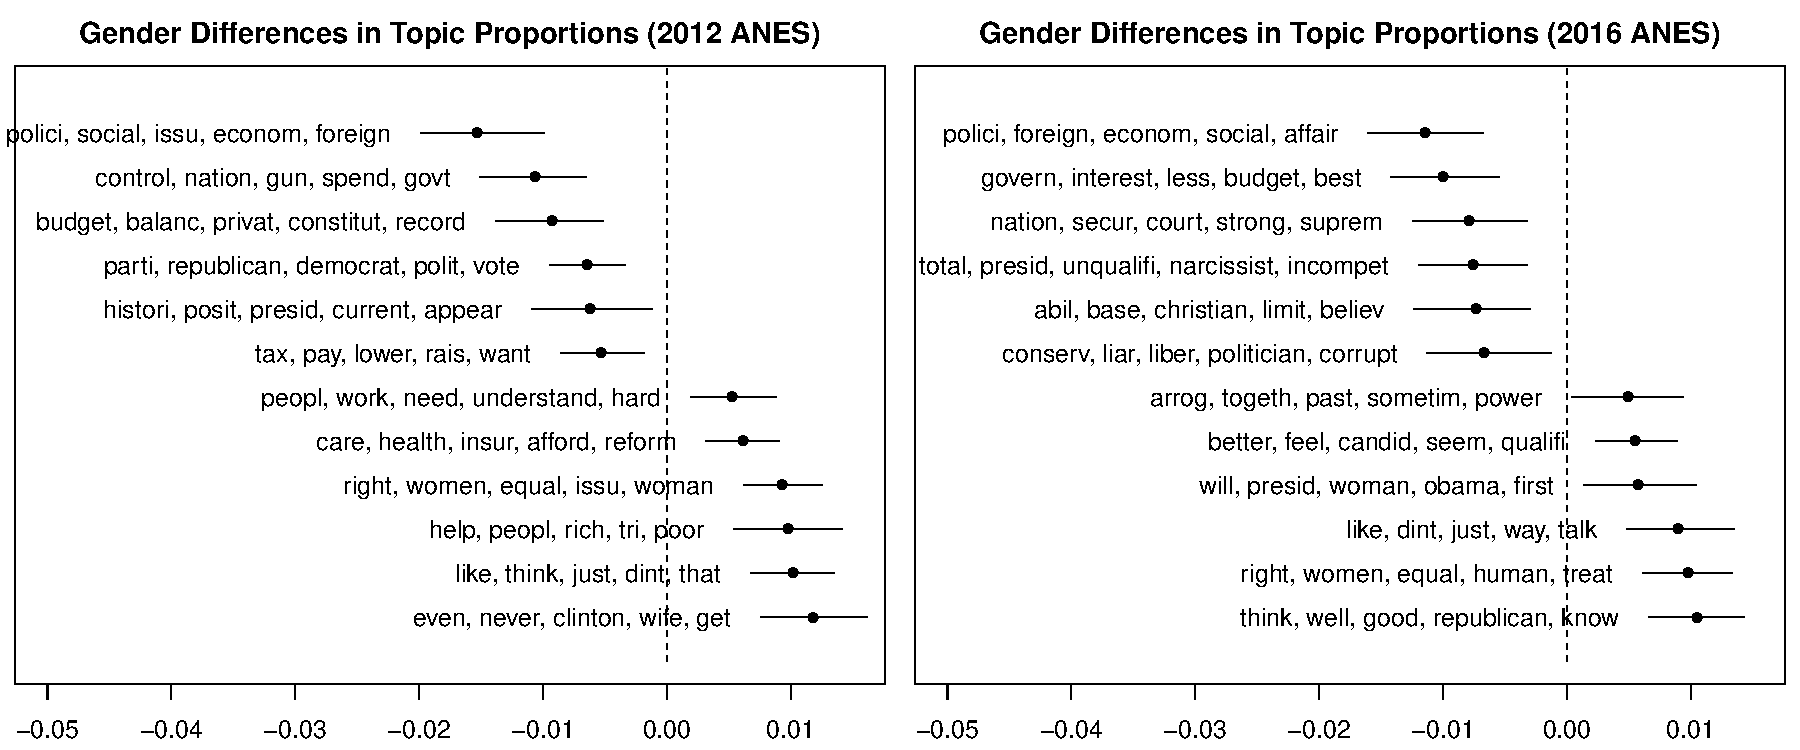
\includegraphics[width=\textwidth]{/data/Dropbox/Uni/Projects/2016/knowledge/fig/stm_gender.pdf}
\caption[Gender differences in topic proprtions in open-ended responses]{Gender differences in topic proportions in open-ended responses based on the structural topic model used to compute discursive sophistication (including 95\% confidence intervals). Coefficients indicate the difference in predicted topic prevalence among men and women; positive values indicate higher prevalence among women. Labels are based on the five highest probability terms related to the topic.
%Full model results are displayed in the appendix, Table~\ref{tab:determinants}
}\label{fig:stm_gender}
\end{figure}

Positive coefficients indicate that women are more likely than men to mention a given topic, and vice versa. As such, the top six topics are more prevalent among men and the bottom six have a higher probability to be mentioned by women. Each coefficient is labeled with the five highest probability terms related to the topic to illustrate its content. Across both ANES studies, women were less likely than men to discuss foreign affairs, economic issues, or the Supreme Court. Instead, they focused on issues related to women's rights, equality, or health care. The considerations taken into account by women when discussing their political preferences are therefore clearly different from men's and---crucially---the issues raised by men happen to be more aligned with what political scientists often deem as necessary information (i.e., pertaining to the economy, institutions, elites, etc.). Yet, from a normative perspective, there is no reason to assume that one set of issues should be more important for citizens when forming their political preferences and making competent voting decisions.

% TODO: elaborate on the explanations for the lack of the gender gap


\section*{Conclusion}
% What is a competent citizen? One who has good reasons for his or her attitudes... we can measure that when examining how repondents talk about their political beliefs.

Political scientists should worry less about pure levels of \textit{factual knowledge} and instead focus on the necessary conditions for individuals to make \textit{competent} decisions. Competence in the context of political decision-making and voting requires citizens to hold informed attitudes about their representatives. Factual knowledge about political institutions might be a useful proxy for competence in certain scenarios. However, it cannot address directly whether individuals hold well-considered opinions about political actors they try to hold accountable. In comparison, the measure of discursive sophistication proposed here is agnostic about the specific contents of people's beliefs, but directly captures the complexity of individual attitude expression. Furthermore, it can be easily applied to assess sophistication in any decision-making context (such as a policy referendum or a local election) by fielding targeted open-ended questions related to the relevant underlying beliefs and preferences.

The findings presented in this paper show that conventional knowledge indices and the discursive measure share a substantial amount of variance. However, they are far from being identical and capture different aspects of sophistication. Most importantly, using the discursive measure, evidence for the gender gap commonly reported using factual knowledge scales disappears. Women might know fewer facts about political institutions, but they do not differ substantively in the complexity of their expressed political beliefs. The fact that women perform just as well as men on discursive sophistication across various surveys can be attributed to the fact that they focus on different considerations when evaluating political parties and candidates. This issue has long been recognized in the literature \citep[e.g.,][]{graber2001processing,dolan2011women}, but it cannot be properly addressed while relying exclusively on off-the-shelf political knowledge batteries. As discussed at the outset, \citet{zaller1992nature} and others made the argument that testing for factual information provides the best measure of political awareness as it captures ``what has actually gotten into people's minds, which, in turn, is critical for intellectual engagement with politics'' (21). The results presented in this paper suggest that a direct examination of open-ended responses provides a viable alternative approach.

% DISCUSS: highlight the advantages of the measure, also regarding the ability to find policy areas that are less gender biased.

% DISCUSS: mention disadvantages of the method, clearly state that it is not to be viewed as a replacement but rather a substitute for political knowledge questions.

% DISCUSS manual coding as alternative? However, manual coding of open-ended responses as employed by \citet{colombo2016justifications} is not always feasible in the context of large-scale surveys, since it can be labor-intensive and requires extensive contextual knowledge, such as high levels of language proficiency.\footnote{The Swiss surveys in Colombo's \citeyearpar{colombo2016justifications} study were conducted in three different languages: German, French, and Italian.} Furthermore, knowledge assessments can be biased by the level of political agreement between individuals \citep{ryan2011accuracy}. As such, I present an alternative approach that relies on quantitative text-analysis methods and can be applied in multiple contexts and different languages.

%\clearpage
%\singlespacing
\bibliographystyle{/data/Dropbox/Uni/Lit/apsr2006}
\bibliography{/data/Dropbox/Uni/Lit/Literature}

\clearpage
\singlespacing
\renewcommand\thesubsection{\Roman{subsection}}
\counterwithin{figure}{section}
\setcounter{page}{1}
\appendices
\textit{Online Appendix:}\\
\textbf{Let's Talk Politics -- A Naive Approach for Measuring Political Sophistication}

%\thispagestyle{empty}
\startcontents[sections]
\printcontents[sections]{l}{1}{\setcounter{tocdepth}{2}}
\clearpage

%\clearpage
\section*{Overview of Data Sources and Open Ended Items}
% CUTS: This section should start on page 6

Throughout the remainder of this paper, I apply the theoretical framework across multiple surveys fielded in two countries that employed different sets of open-ended questions. Each survey focuses on sophistication in the context of distinct political tasks, namely the evaluation of (1) candidates running for public office, (2) broad issue areas such as health care and gun legislation, and (3) specific legislative policy referenda. The data sets are briefly described below.


\subsection*{2012 \& 2016 American National Election Study}
The main analyses are based on the 2012 and 2016 wave of the American National Election Study (ANES), each of which consists of a representative survey of about 5000 adults in the months before the US Presidential election in each year. About 2000 respondents in each wave participated in face-to-face interviews while the remaining respondents filled out the survey online. For the purpose of the present analyses, I rely on pooled datasets while controlling for differences in survey mode. Discursive sophistication is evaluated using a set of open-ended questions in which respondents were asked to list anything in particular that they like/dislike about the Democratic/Republican party as well as anything that might make them vote/not vote for either of the Presidential candidates. They were probed by the interviewer asking ``anything else?'' until the respondent answered ``no.'' Overall, there are a total number of 8 open-ended responses where individuals described their beliefs and attitudes towards political actors. Individuals who did not respond to all of the open-ended items (420 in 2012; 204 in 2016), or who responded in Spanish (228 in 2012; 43 in 2016), are excluded from the analysis since discursive sophistication for them is not directly comparable to the remaining respondents.


% TODO: add footnote again after reviews
\subsection*{2015 YouGov Survey}
In order to replicate and extend the main analyses, I rely on a separate nationally representative survey employing an alternative set of open-ended responses. The data was collected by YouGov in December 2015 and contains responses of 1000 U.S. citizens. %\footnote{See \citet{clifford2018disgust} for details on the study.} 
As part of this study, respondents were asked to describe their attitudes towards two prominent political issues that were discussed frequently in the media. First, they were asked in a closed format whether they favor or oppose stricter gun laws. Subsequently, they were asked to respond to the following two questions:
\begin{itemize}\setlength\itemsep{0em}
	\item Still thinking about the question you just answered, what thoughts came to mind while you were answering that question? Please try to list everything that came to mind.
	\item Thinking about the mass shootings that have occurred in the U.S. in the last few years, what factors do you think are responsible for the shootings?
\end{itemize}
Second, the respondents reported on their attitudes towards the Affordable Care Act in a closed format and were then asked to elaborate in their own words by answering the following questions:
\begin{itemize}\setlength\itemsep{0em}
	\item Still thinking about the question you just answered, what thoughts came to mind while you were answering that question? Please try to list everything that came to mind.
	\item For decades, experts have observed that the United States spends far more per person on health care than any other country. However, the U.S. falls behind on most measures of health care outcomes, such as life expectancy. What factors do you think are responsible for the state of our health care system?
\end{itemize}
%Here, discursive sophistication is evaluated based on the verbatim responses to the four preceding questions using the same procedures described above. 
Compared to the open-ended likes/dislikes items included in the 2012 and 2016 ANES, the questions directly address considerations related to specific policy issues that were prominent in the political discourse at the time of the survey. Respondents who did not provide an answer to all of the open-ended questions were removed from the analysis (48).


\subsection*{Swiss Referendum Survey}
Lastly, I examine survey data on Swiss citizens justifying their vote choices on multiple referenda used in a recent analysis by \citet{colombo2016justifications}. The author compiled a data set of cross-sectional surveys administered in Switzerland after national popular votes on multiple policy propositions. The original surveys were conducted as representative samples after each of thirty-four national policy votes that were held between 2008 and 2012 resulting in a total of about 27,000 observations. However, respondents were only asked to justify their decision for or against a given proposition in verbatim if they participated in the vote in the first place. As such, about 5,000 individuals in the data set did not provide an open-ended response. The remaining respondents were asked to describe the main reason as well as additional justifications for their decision in two separate items. As before, discursive sophistication is evaluated based on verbatim responses to both questions. Since the Swiss survey was conducted in three different languages (German, French, and Italian), I computed the measure of discursive sophistication separately for each group of respondents.
% QUESTION wording for Swiss study?

\section[Information on Discursive Sophistication Components]{Detailed Information on Open-Ended Responses and Discursive Sophistication Components}\label{app:oeinfo}
%\renewcommand\thefigure{A.\arabic{figure}}
%\renewcommand\thetable{A.\arabic{table}}
%\setcounter{figure}{0}
%\setcounter{table}{0}


\subsection{Distribution of Word Counts in Open-Ended Responses}

\begin{figure*}[h]
    \centering
    \begin{subfigure}[t]{0.49\textwidth}
        \centering
        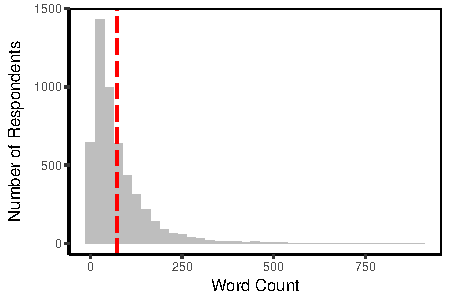
\includegraphics{/data/Dropbox/Uni/projects/2016/knowledge/fig/anes2012_wc.pdf}
        \caption{2012 ANES}
    \end{subfigure}%
	\begin{subfigure}[t]{0.49\textwidth}
        \centering
        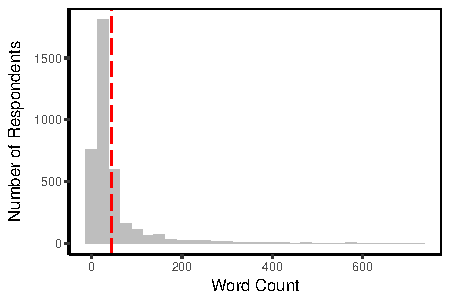
\includegraphics{/data/Dropbox/Uni/projects/2016/knowledge/fig/anes2016_wc.pdf}
        \caption{2016 ANES}
    \end{subfigure}%
    
    \begin{subfigure}[t]{0.49\textwidth}
        \centering
        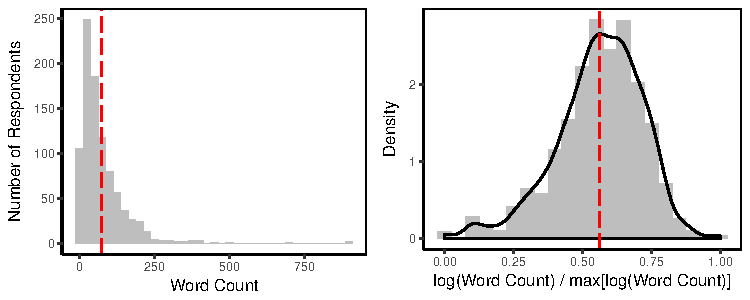
\includegraphics{/data/Dropbox/Uni/projects/2016/knowledge/fig/yg_wc.pdf}
        \caption{2015 YouGov}
    \end{subfigure}
    \begin{subfigure}[t]{0.49\textwidth}
         \centering
         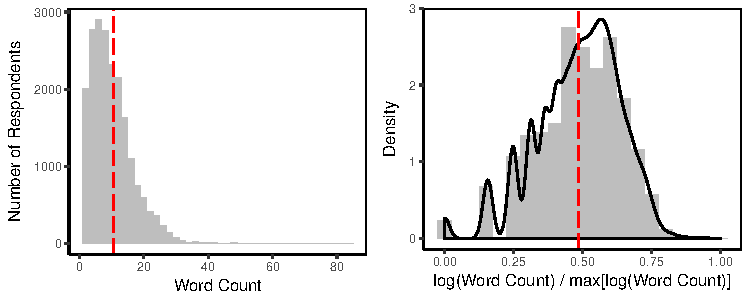
\includegraphics{/data/Dropbox/Uni/projects/2016/knowledge/fig/swiss_wc.pdf}
         \caption{Swiss Survey}
    \end{subfigure}
    \caption[Histograms of total word count in open-ended responses]{Histograms of total word count in the collection of open-ended responses for each individual. The dashed red lines indicate the average response lengths in each survey.}\label{fig:wc}
\end{figure*}


\clearpage
\subsection{Overview of Topic Proportions}

\begin{figure}[h]\centering
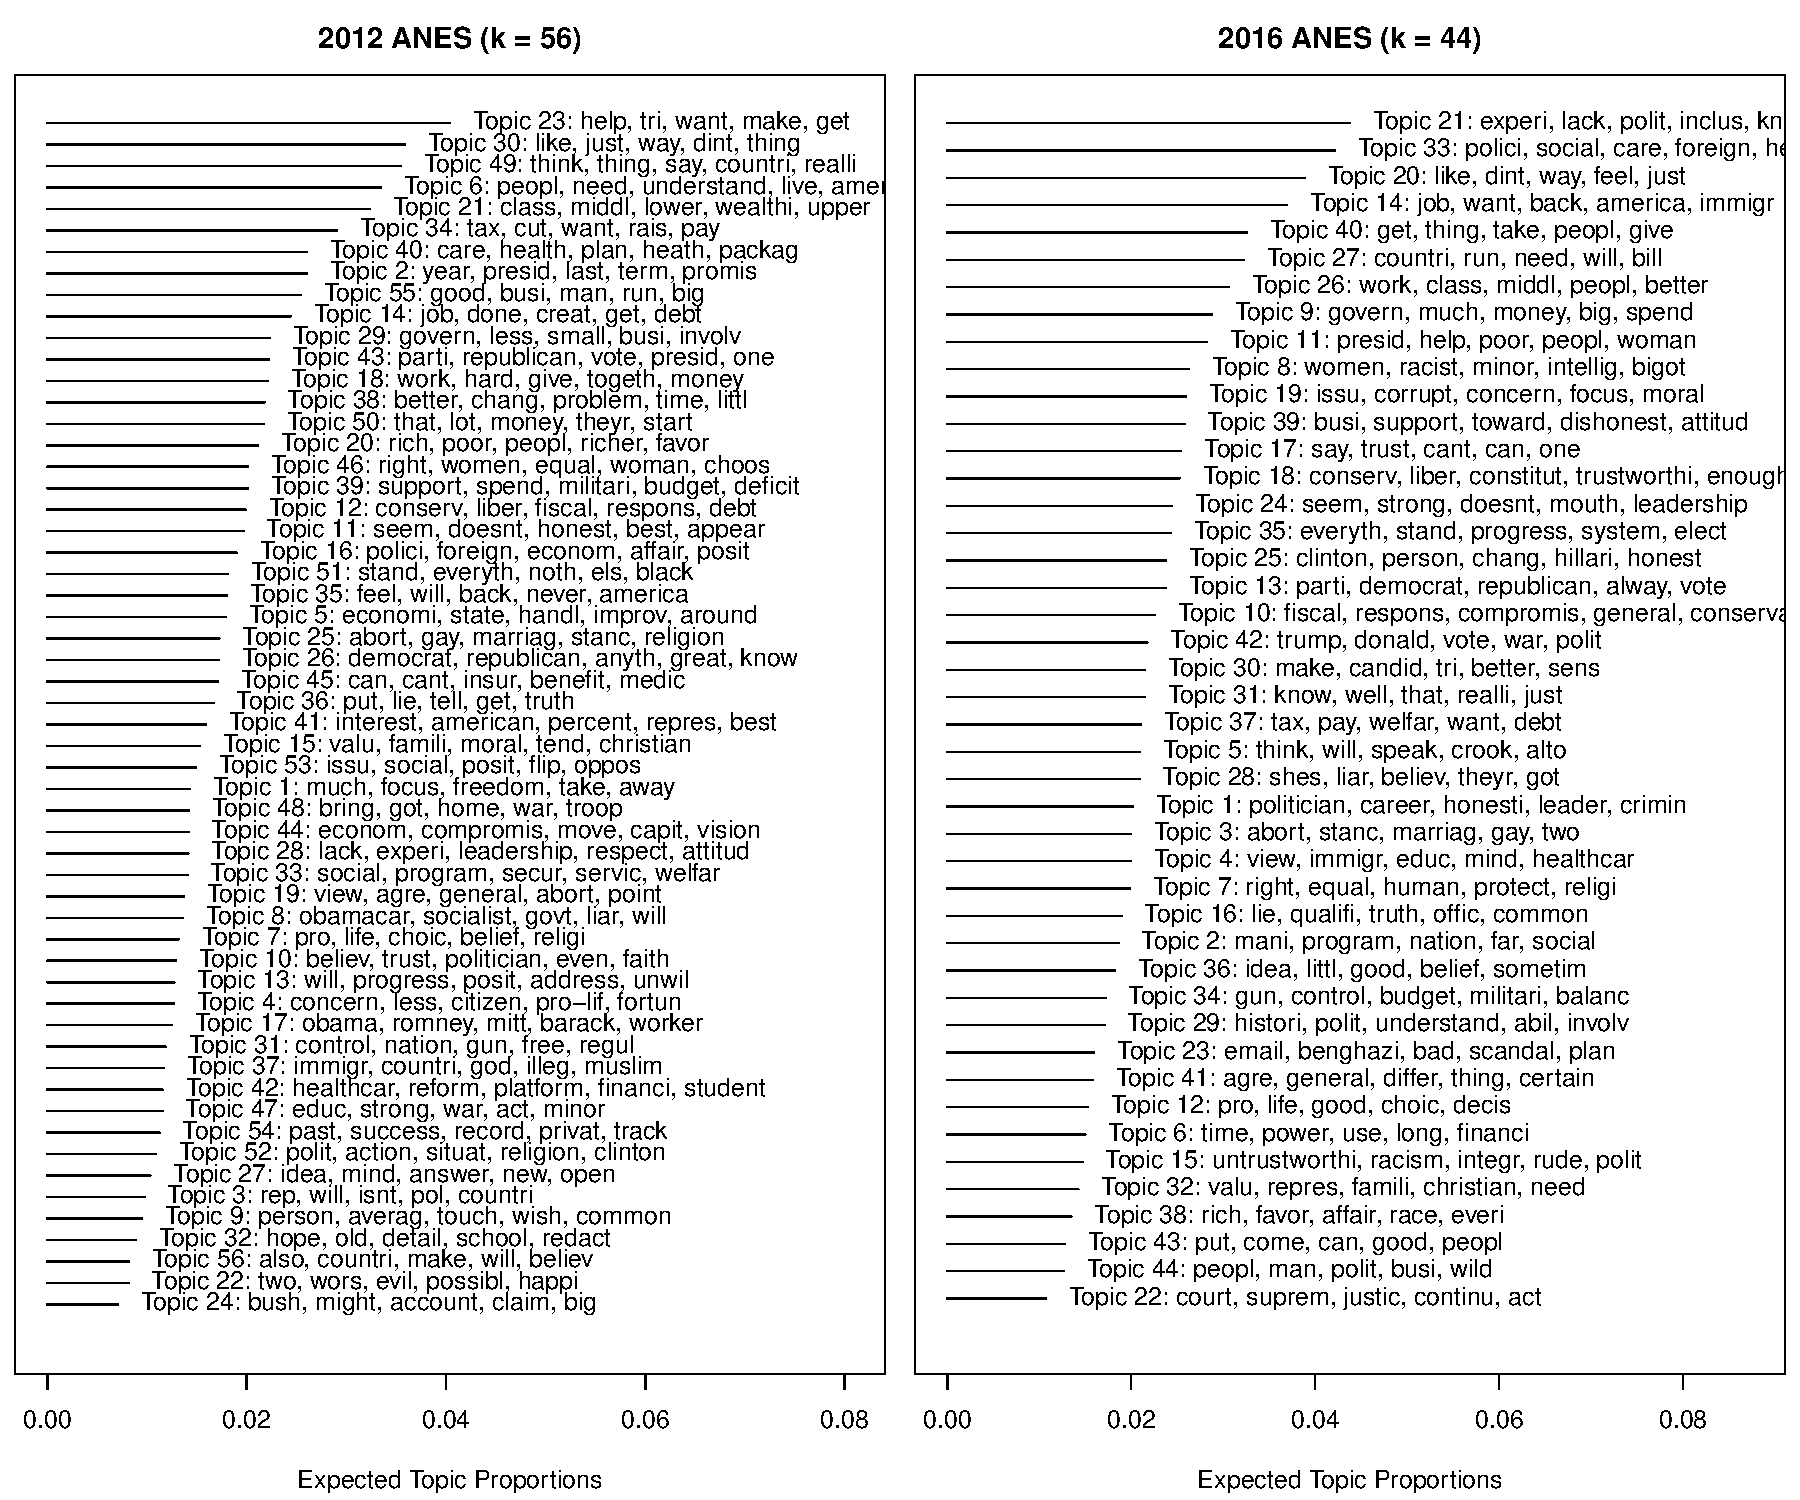
\includegraphics[width=\textwidth]{/data/Dropbox/Uni/projects/2016/knowledge/fig/anes_stm_prop.pdf}
\caption[Estimated topic proportions in the 2012 and 2016 ANES based on the structural topic model]{Estimated topic proportions in the 2012 and 2016 ANES based on the structural topic model. See Appendix~\ref{app:topicmodel} for details on the model specification.}\label{fig:anes_stm_prop}
\end{figure}

\begin{figure}[h]\centering
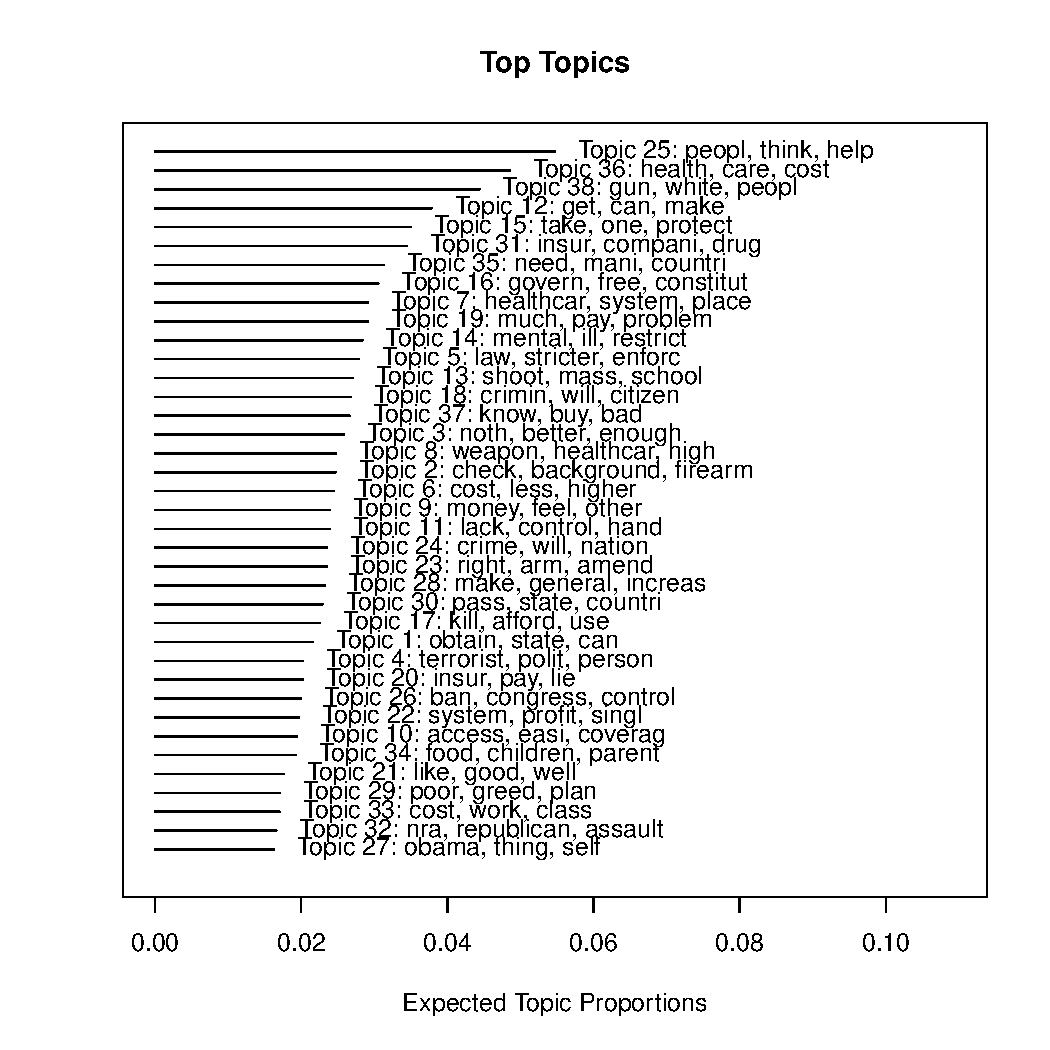
\includegraphics[width=.5\textwidth]{/data/Dropbox/Uni/projects/2016/knowledge/fig/yg_stm_prop.pdf}
\caption[Estimated topic proportions in the 2015 YouGov survey based on the structural topic model]{Estimated topic proportions in the 2015 YouGov survey based on the structural topic model. See Appendix~\ref{app:topicmodel} for details on the model specification.}\label{fig:yg_stm_prop}
\end{figure}

\begin{figure}[h]\centering
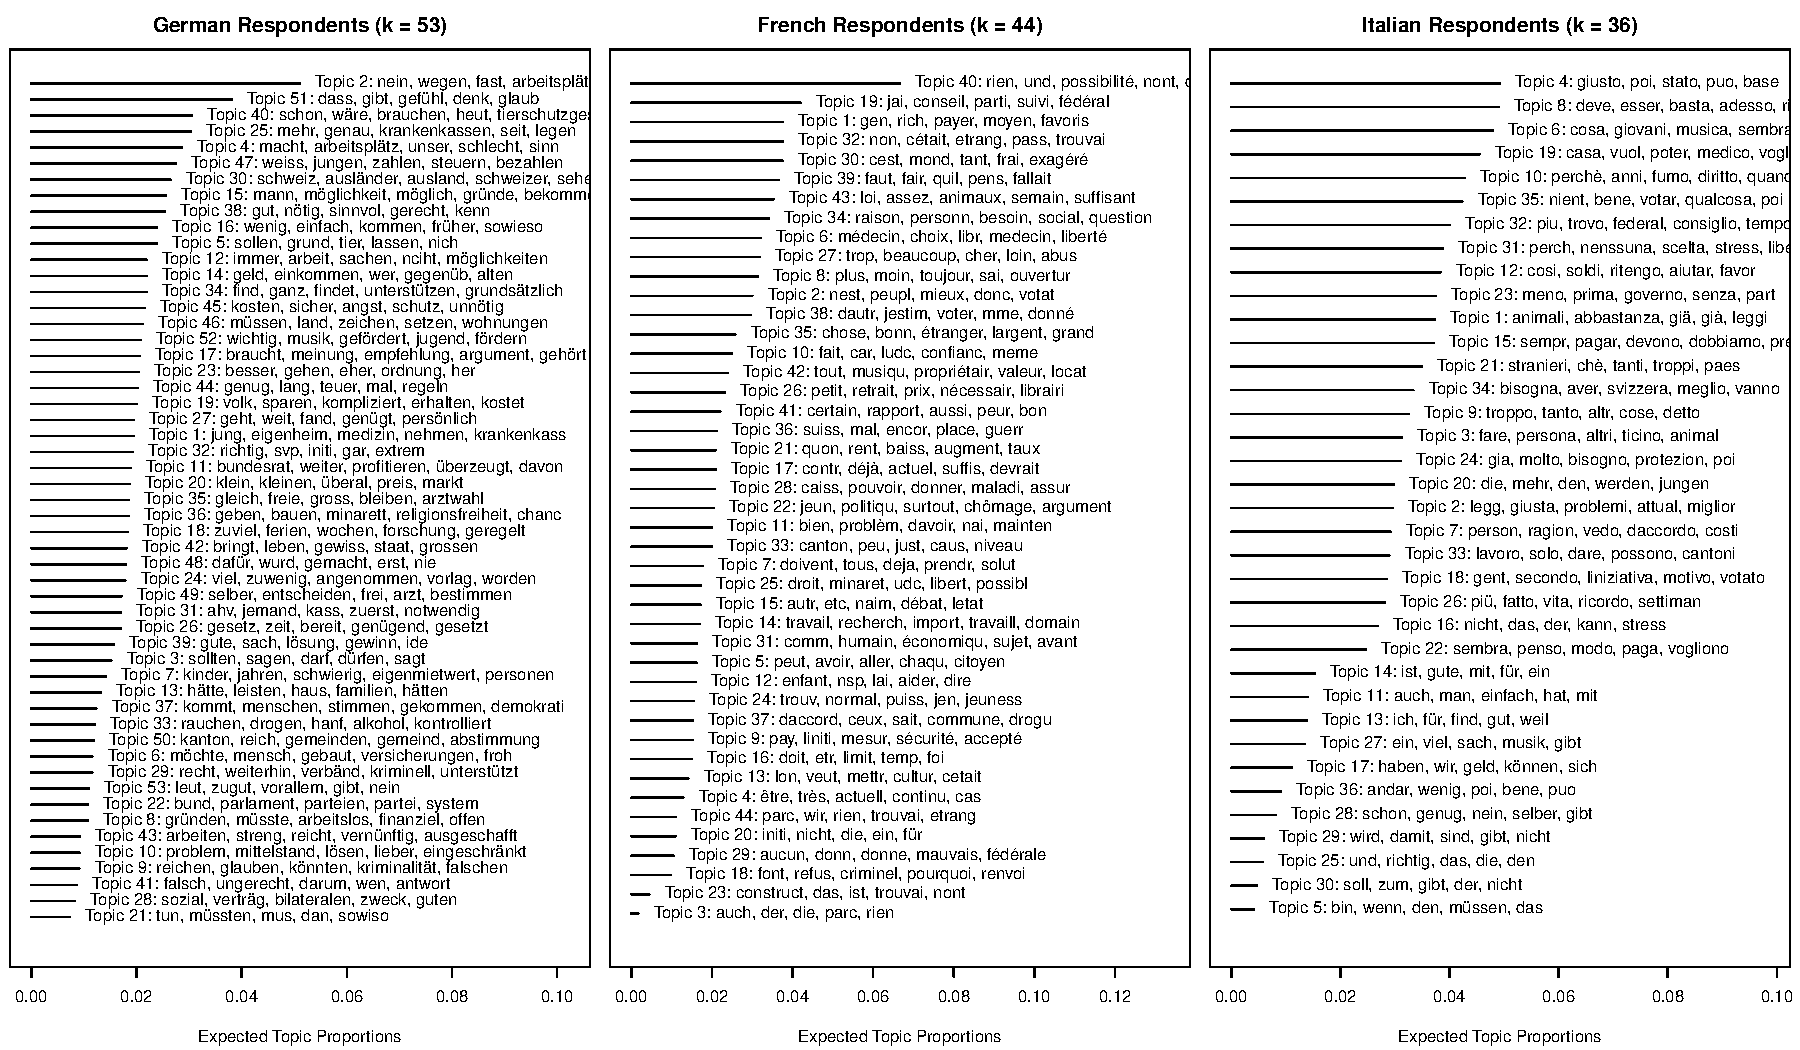
\includegraphics[width=\textwidth]{/data/Dropbox/Uni/projects/2016/knowledge/fig/swiss_stm_prop.pdf}
\caption[Estimated topic proportions in the Swiss survey based on the structural topic model]{Estimated topic proportions in the Swiss survey based on the structural topic model. See Appendix~\ref{app:topicmodel} for details on the model specification.}\label{fig:swiss_stm_prop}
\end{figure}


\clearpage
\subsection{Discursive Sophistication Components}
\begin{figure*}[h]
    \centering
    \begin{subfigure}[h]{0.4\textwidth}
        \centering
        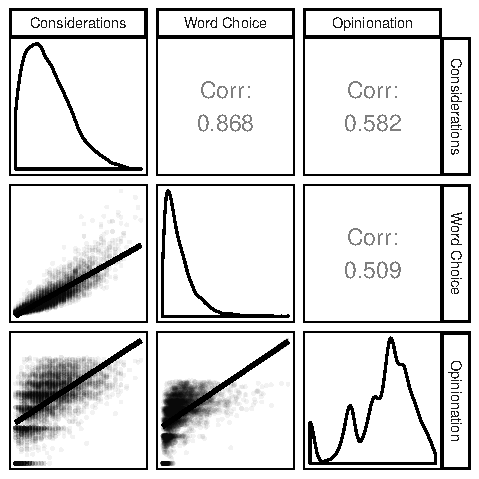
\includegraphics{/data/Dropbox/Uni/projects/2016/knowledge/fig/anes2012_corplot_components.pdf}
        \caption{2012 ANES}
    \end{subfigure}%
    \begin{subfigure}[h]{0.4\textwidth}
         \centering
         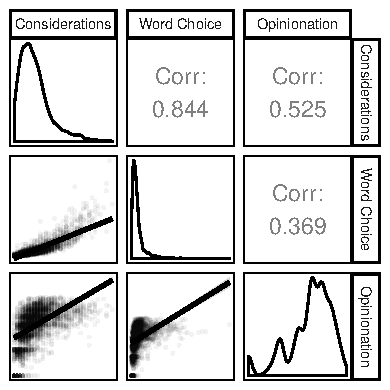
\includegraphics{/data/Dropbox/Uni/projects/2016/knowledge/fig/anes2016_corplot_components.pdf}
         \caption{2016 ANES}
    \end{subfigure}%
    
    \begin{subfigure}[h]{0.4\textwidth}
        \centering
        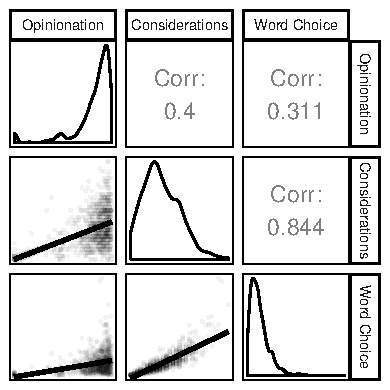
\includegraphics{/data/Dropbox/Uni/projects/2016/knowledge/fig/yg_corplot_components.pdf}
        \caption{2015 YouGov}
    \end{subfigure}%
    \begin{subfigure}[h]{0.4\textwidth}
         \centering
         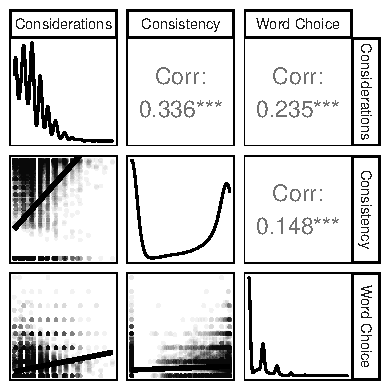
\includegraphics{/data/Dropbox/Uni/projects/2016/knowledge/fig/swiss_corplot_components.pdf}
         \caption{Swiss Survey}
    \end{subfigure}
    \caption[Correlation matrix of individual components of discursive sophistication.]{Correlation matrix of individual components of discursive sophistication. The plots on the diagonal display univariate densities for each component. The panels in the lower triangular display the scatter plot of two measures as well as a linear fit. %The upper triangular displays the correlation coefficient.
     }\label{fig:components}
\end{figure*}


\clearpage
\section{Pre-Processing and Topic Model Specification}\label{app:topicmodel}
%\renewcommand\thefigure{B.\arabic{figure}}
%\renewcommand\thetable{B.\arabic{table}}
%\setcounter{figure}{0}
%\setcounter{table}{0}

\subsection{PreText Analysis}
Two components of discursive sophistication (\textit{considerations} and \textit{word choice}) rely on quantities extracted from structural topic models \citep{roberts2014structural}. As with any other text-as-data approach, a necessary first step before estimating the topic model is to pre-process the raw text and convert it into a document term matrix \citep[DTM, see for example][]{manning2008introduction}. Common pre-processing procedures include stemming and lowercasing, as well as the removal of numbers, punctuation, stopwords, and infrequent terms. However, topic models and other unsupervised learning techniques can be sensitive to these pre-processing choices \citep[c.f.,][]{denny2018text}. To address this issue, \citet{denny2018text} recommend that researchers compare DTMs under all possible pre-processing regimes. The authors propose \textit{preText scores} as a measure to quantify the extent to which varying pre-processing regimes may yield unusual results compared to a baseline without any pre-processing.

\begin{figure}[h]
\centering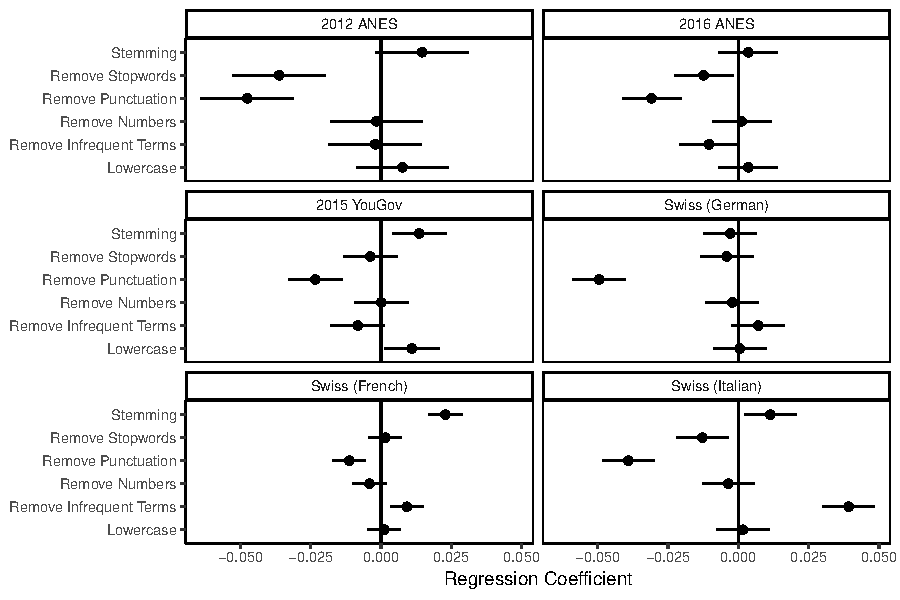
\includegraphics{/data/Dropbox/Uni/projects/2016/knowledge/fig/pretext.pdf}
    \caption[PreText analysis of pre-processing decisions of open-ended responses across all datasets]{PreText analysis of pre-processing decisions of open-ended responses across all datasets. Regression coefficients display the effects of each of the six pre-processing choices on the resulting preText score.}\label{fig:pretext}
\end{figure}

\clearpage
\subsection{Robustness Checks for Varying Model Specifications}

Following the procedure outlined in \citet{denny2018text}, Figure~\ref{fig:pretext} displays the results of a linear model regressing preText scores resulting from all possible pre-processing regimes on each individual step for a random subset of 500 open-ended responses in each of the studies included in the analyses. Significant coefficients indicate that the topic model results may be sensitive to the respective pre-processing step. As such, removing stopwords and punctuation, as well as removing infrequent terms (at least in the 2016 ANES) might be problematic. \citet{denny2018text}, however, emphasize that the most important consideration in choosing pre-processing steps are theoretical. Given that the purpose of the topic model is to extract considerations related to political preferences, there are strong theoretical reasons to remove stopwords and punctuation from open-ended responses as they do not contain any relevant content. Furthermore, I apply lowercasing and stemming of terms to reduce resulting document term matrix to a computationally more manageable size and since these pre-processing steps should not be influential according to the preText analysis.

It is less obvious from a theoretical perspective whether to remove infrequent terms from open-ended responses, although it is preferred in order to make the estimation of the discursive sophistication components computationally efficient. Since the preText analysis for the 2016 ANES suggests that this pre-processing step might be influential, I compare discursive sophistication for both alternative regimes below \citep[c.f.,][]{denny2018text}. Before turning to this sensitivity check, however, I consider another crucial modeling choice when working with topic models: determining the total number of topics $k$ to be estimated. For all analyses reported below, the number of topics was selected using the algorithm proposed by \citet{lee2014low} and implemented in the \texttt{stm} package in \textbf{R} \citep{roberts2014stm}.

\begin{figure}[h]\centering
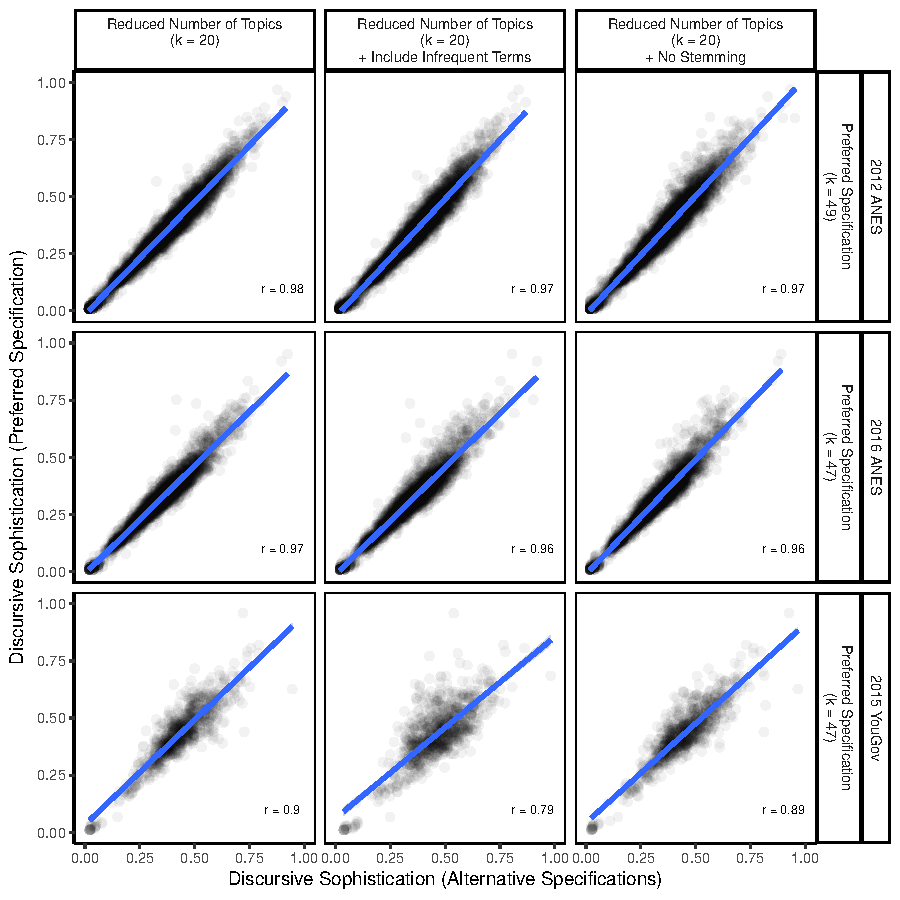
\includegraphics{/data/Dropbox/Uni/projects/2016/knowledge/fig/pretext_robustness.pdf}
\caption[Robustness of discursive sophistication measure for different pre-processing choices and topic model specifications]{Robustness of discursive sophistication measure for different pre-processing choices and topic model specifications.}\label{fig:pretext_robustness}
\end{figure}

Figure~\ref{fig:pretext_robustness} examines whether the proposed measure of discursive sophistication is sensitive to the removal of infrequent terms as well as the chosen number of topics $k$. The y-axis depicts the preferred pre-processing regime including all steps discussed above while the x-axis plots results for alternative specifications. The panels on the left compare the preferred specification to discursive sophistication based on a reduced number of topics ($k=20$). The middle panels additionally include infrequent terms instead of removing them.\footnote{Calculating discursive sophistication with large numbers of topics while including infrequent terms is computationally prohibitive.} The panels on the right do not perform stemming as part of the pre-processing step. Across all panels, discursive sophistication scores are highly correlated and therefore insensitive to pre-processing choices and varying numbers of topics.

In summary, open-ended responses in the analyses reported in the main text are pre-processed by stemming and lowercasing, as well as the removing numbers, punctuation, stopwords, and infrequent terms (i.e., terms that appear in fewer than 10 responses).\footnote{Prior to applying these pre-processing steps, open-ended responses in the 2012 \& 2016 ANES as well as the 2015 YouGov survey are cleaned by correcting spelling errors using an implementation of the Aspell spell-checking algorithm (\url{www.aspell.net}).} While the results discussed in the manuscript are based on this preferred specification, the substantive results are robust for alternative pre-processing regimes or varying numbers of topics.


\clearpage
\section{Additional Information on Remaining Variables}\label{app:variables}
%\renewcommand\thefigure{C.\arabic{figure}}
%\renewcommand\thetable{C.\arabic{table}}
%\setcounter{figure}{0}
%\setcounter{table}{0}

\subsection{Item Selection and Recoding}

\paragraph{Conventional measures of political knowledge:}
\begin{itemize}
\item \textit{2012 ANES}: Additive index of correct responses to 5 knowledge items included in the pre-election wave (number of Presidential terms, size of budget deficit, length of Senate term, meaning of Medicare, federal government spending). `Don't know' responses are considered incorrect. Interviewer evaluations are based on the assessment of the respondent's general level of information about politics recorded at the end of the pre-election wave.
\item \textit{2016 ANES}: Additive index of correct responses to 4 knowledge items included in the pre-election wave (length of Senate term, federal government spending, majority in House, majority in Senate). `Don't know' responses are considered incorrect. Interviewer evaluations are based on the assessment of the respondent's general level of information about politics recorded at the end of the pre-election wave.
\item \textit{2015 YouGov Survey}: Additive index of correct responses to 8 knowledge items (Speaker of the House, meaning of TPP, Chair of Federal Reserve Board, current unemployment rate, Presidential veto override, meaning of Common Core, leading source of electricity in US, majority in Senate). `Don't know' responses are considered incorrect.
\end{itemize}

\paragraph{Dependent variables:}
\begin{itemize}
\item \textit{Turnout} (2012 \& 2016 ANES): Dichotomous indicator, based on post-election wave.
\item \textit{Non-conventional participation} (2012 \& 2016 ANES): Additive index of different forms of political engagement (participated in protest, signed petition, wore campaign button, wrote letter to public official).
\item \textit{Internal efficacy} (2012 \& 2016 ANES): Sum of two agree/disagree items (politics too complicated, good understanding of political issues [reversed]).
\item \textit{External efficacy} (2012 \& 2016 ANES): Sum of two agree/disagree items (public officials don't care, people have no say about what the government does).
\item \textit{Information retrieval (2015 YouGov Survey)}: Additive index of correct answers to 9 questions about the fictional disease described in the news article (symptoms: fatigue, headaches, diarrhea, joint pain, boils, warts, fever; virus spread; cure for the virus)
\item \textit{Candidate policy positions} (2012 \& 2016 ANES): Placement of Republican and Democratic Presidential candidates on 7-point scale (ideology, government spending, defense spending, insurance policy, job guarantee, aid to Blacks, environment vs jobs).
%\item \textit{Correct voting} (2012 \& 2016 ANES): Dichotomous indicator created according to the procedures described in \citet{lau1997voting,lau2008exploration} and \citet{sokhey2012social}. Correct votes are determined by party identification, overlap in issue positions (see above), and attachments to social groups that are aligned with each candidate. All components are weighted equally. Overlap in issue positions is conceptualized using directional voting scores \citep{rabinowitz1989directional}, where ``true'' candidate positions are determined by averaging perceived positions for highly knowledgeable respondents (scoring above median factual knowledge). Social groups (e.g., middle class, unions, tea party, etc.) are viewed as aligned with a candidate if group attachment differs significantly and in direction between highly knowledgeable (above median factual knowledge) supporters of each candidate (i.e., knowledgeable supporters of one group view them negatively on average while knowledgeable supporters of the other group view them positively on average).
\end{itemize}

\paragraph{Control variables:}
\begin{itemize}
\item \textit{Gender} (2012 \& 2016 ANES, 2015 YouGov Survey): Dichotomous indicator for female respondents.
\item \textit{Wordsum vocabulary scores}  (2012 \& 2016 ANES): Modified version of the GSS wordsum vocabulary test consisting of 10 terms.
\item \textit{Media exposure} (2012 \& 2016 ANES): Additive index of the frequency of weekly exposure to various political information sources such as newspapers or TV news (2012 ANES). In the 2016 ANES, it only consists of a single item measuring the number of days in the past week the respondent has spent watching/reading/listening news on any media.
\item \textit{Political discussion frequency} (2012 \& 2016 ANES): Self-reported count of days in the past week spent discussing politics with family or friends.
\item \textit{College education} (2012 \& 2016 ANES, 2015 YouGov Survey): Dichotomous indicator for Bachelor's degree or higher.
\item \textit{Family/Household income} (2012 \& 2016 ANES, 2015 YouGov Survey): Self-reported household income categories.
\item \textit{Age} (2012 \& 2016 ANES, 2015 YouGov Survey): Logged age in years.
\item \textit{Race} (2012 \& 2016 ANES, 2015 YouGov Survey): Dichotomous indicator for black non-Hispanic vs. others.
\item \textit{Church attendance} (2012 \& 2016 ANES, 2015 YouGov Survey): Six-category indicator of the frequency of church attendance. 
\item \textit{Survey Mode} (2012 \& 2016 ANES): Dichotomous indicator for face-to-face vs. online samples of the ANES surveys.
\item \textit{Personality characteristics} (2012 \& 2016 ANES): Measures of extraversion and being reserved, part of the Ten Item Personality Inventory (TIPI) measuring the ``Big Five'' personality traits.
\item \textit{Response length} (2012 \& 2016 ANES): Logged number of words in the collection of open-ended responses by each individual.
\end{itemize}


\clearpage
\subsection{Variable Distributions -- 2012 ANES}
\begin{figure}[h]\centering
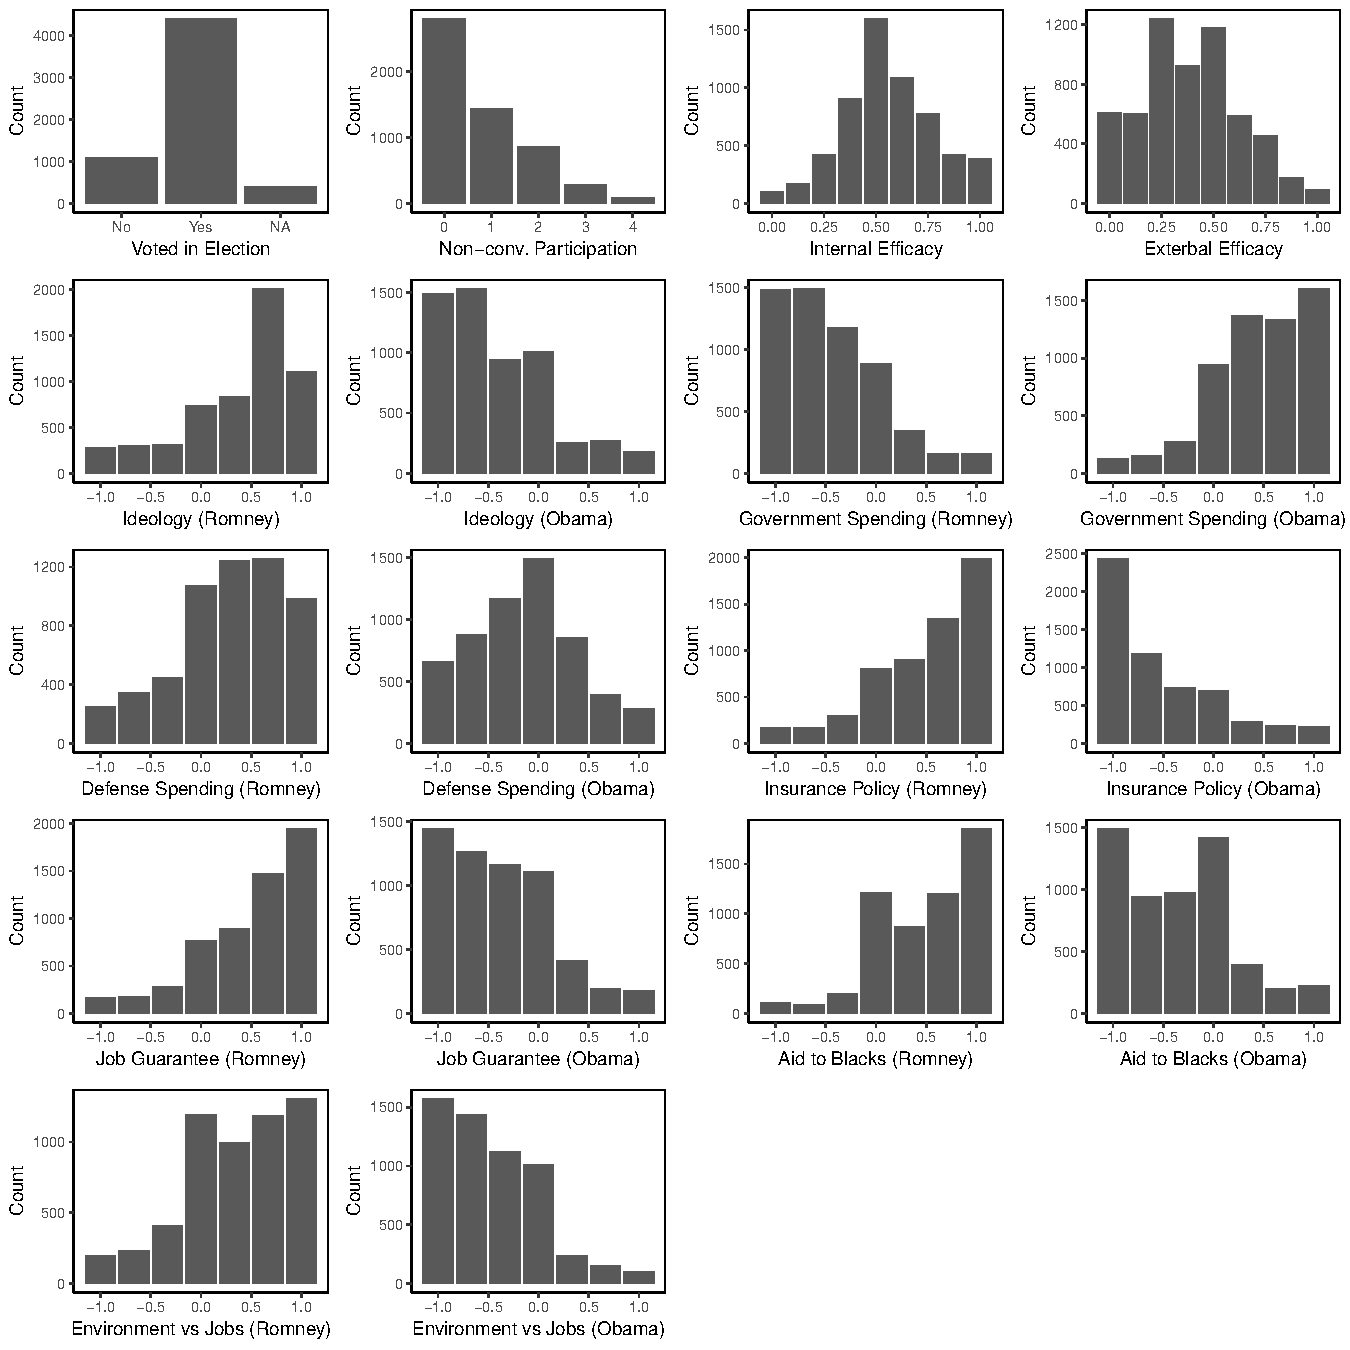
\includegraphics[width=\textwidth]{/data/Dropbox/Uni/projects/2016/knowledge/fig/descriptives_anes2012dv.pdf}
\caption[Histograms of dependent variables included in 2012 ANES]{Histograms of dependent variables included in 2012 ANES.}\label{fig:descriptives_anes2012dv}
\end{figure}

\begin{figure}[h]\centering
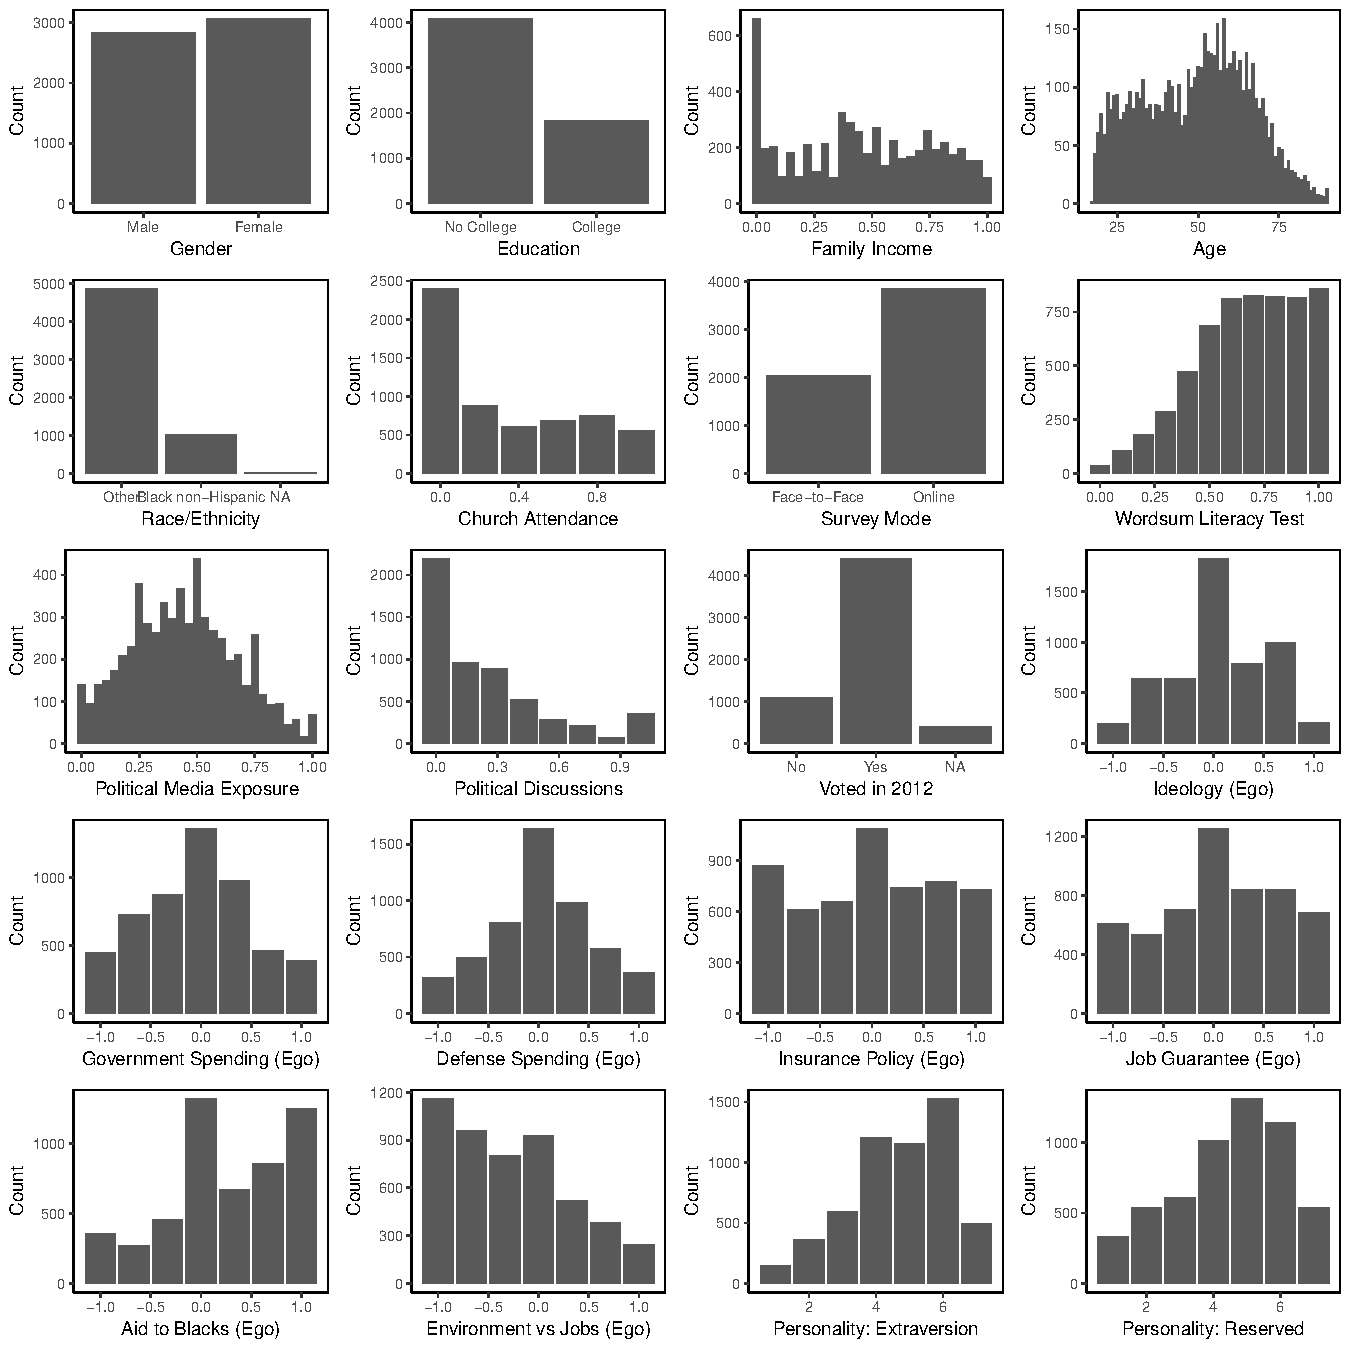
\includegraphics[width=\textwidth]{/data/Dropbox/Uni/projects/2016/knowledge/fig/descriptives_anes2012iv.pdf}
\caption[Histograms of independent variables included in 2012 ANES]{Histograms of independent variables included in 2012 ANES.}\label{fig:descriptives_anes2012iv}
\end{figure}

\clearpage
\subsection{Variable Distributions -- 2016 ANES}
\begin{figure}[h]\centering
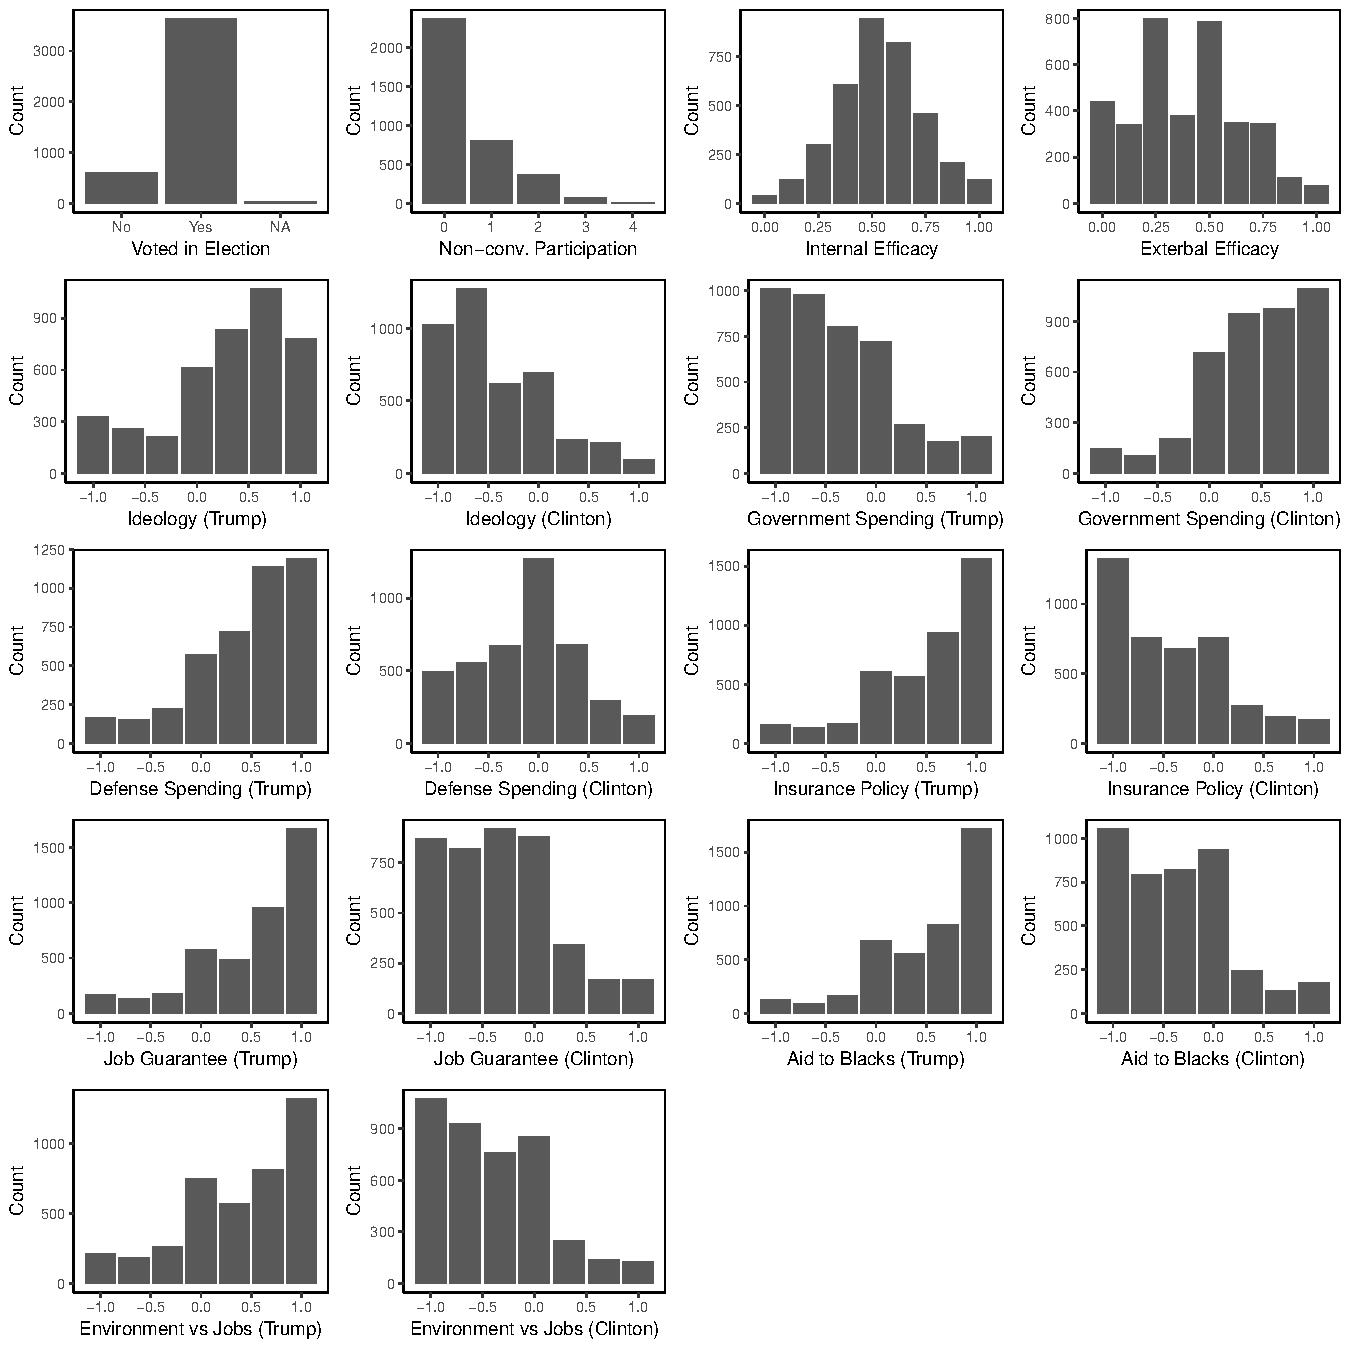
\includegraphics[width=\textwidth]{/data/Dropbox/Uni/projects/2016/knowledge/fig/descriptives_anes2016dv.pdf}
\caption[Histograms of dependent variables included in 2016 ANES]{Histograms of dependent variables included in 2016 ANES.}\label{fig:descriptives_anes2016dv}
\end{figure}

\begin{figure}[h]\centering
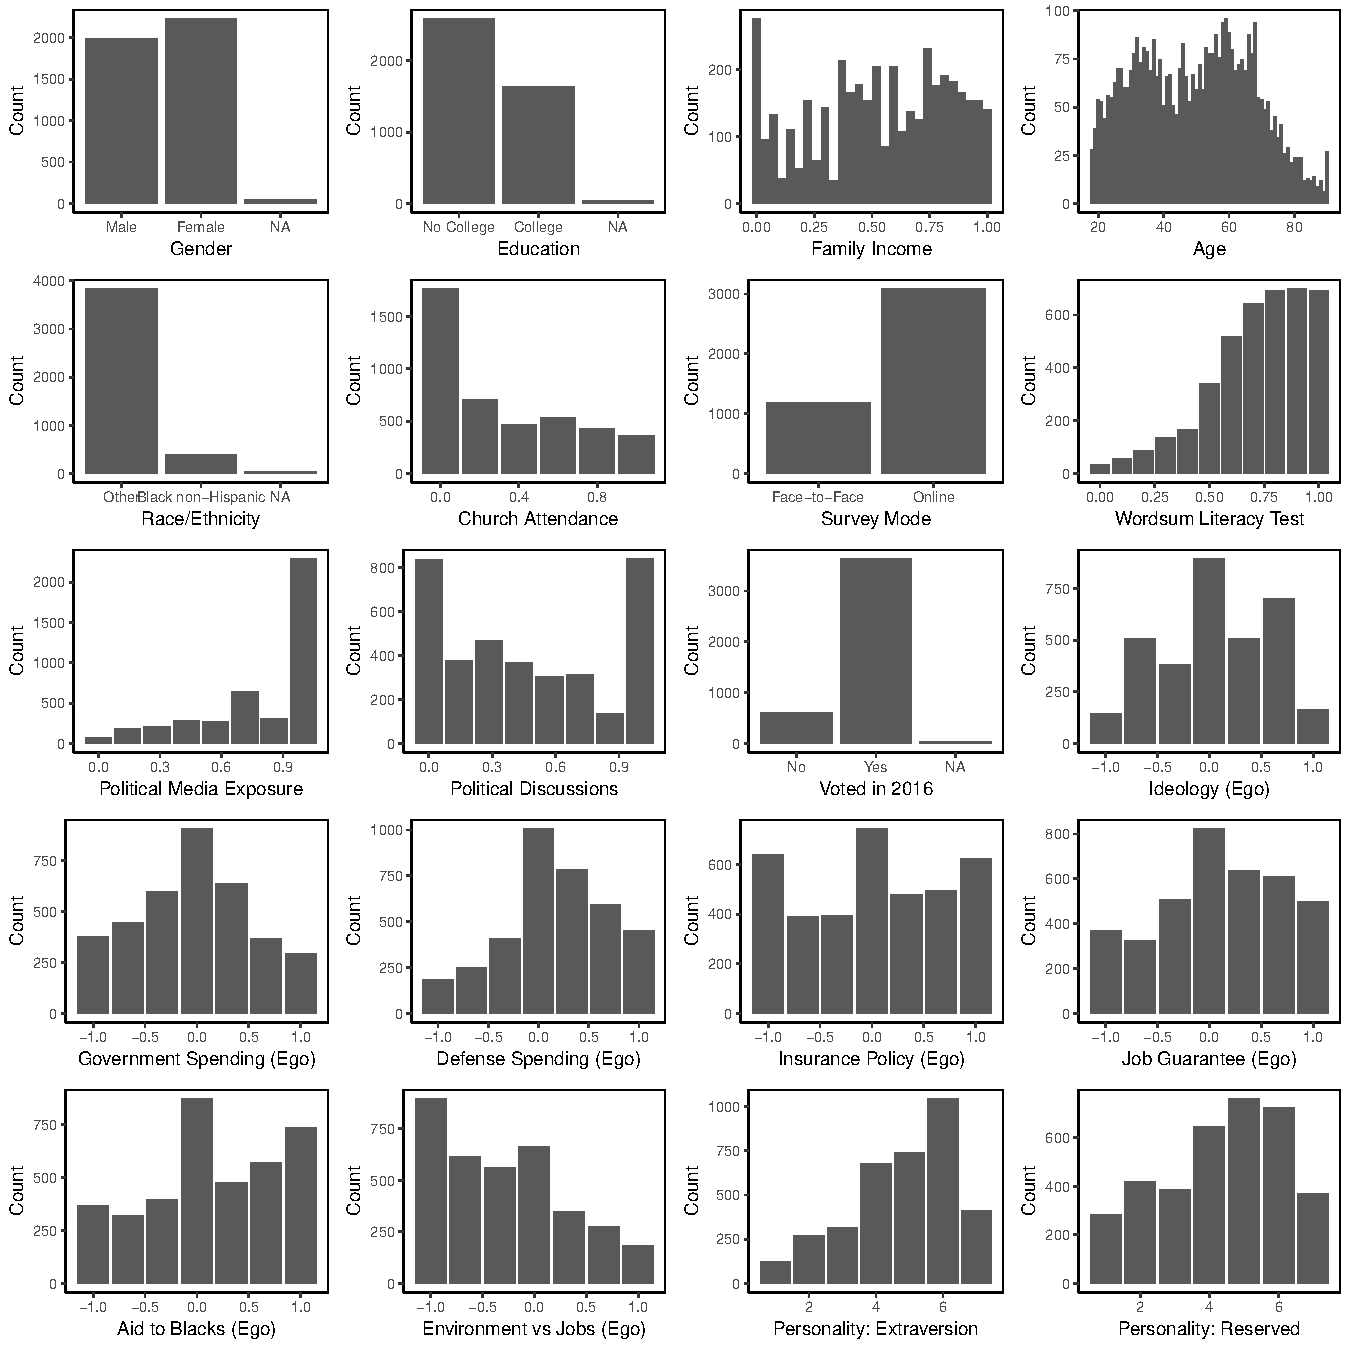
\includegraphics[width=\textwidth]{/data/Dropbox/Uni/projects/2016/knowledge/fig/descriptives_anes2016iv.pdf}
\caption[Histograms of independent variables included in 2016 ANES]{Histograms of independent variables included in 2016 ANES.}\label{fig:descriptives_anes2016iv}
\end{figure}

\clearpage
\subsection{Variable Distributions -- 2015 YouGov}

\begin{figure}[h]\centering
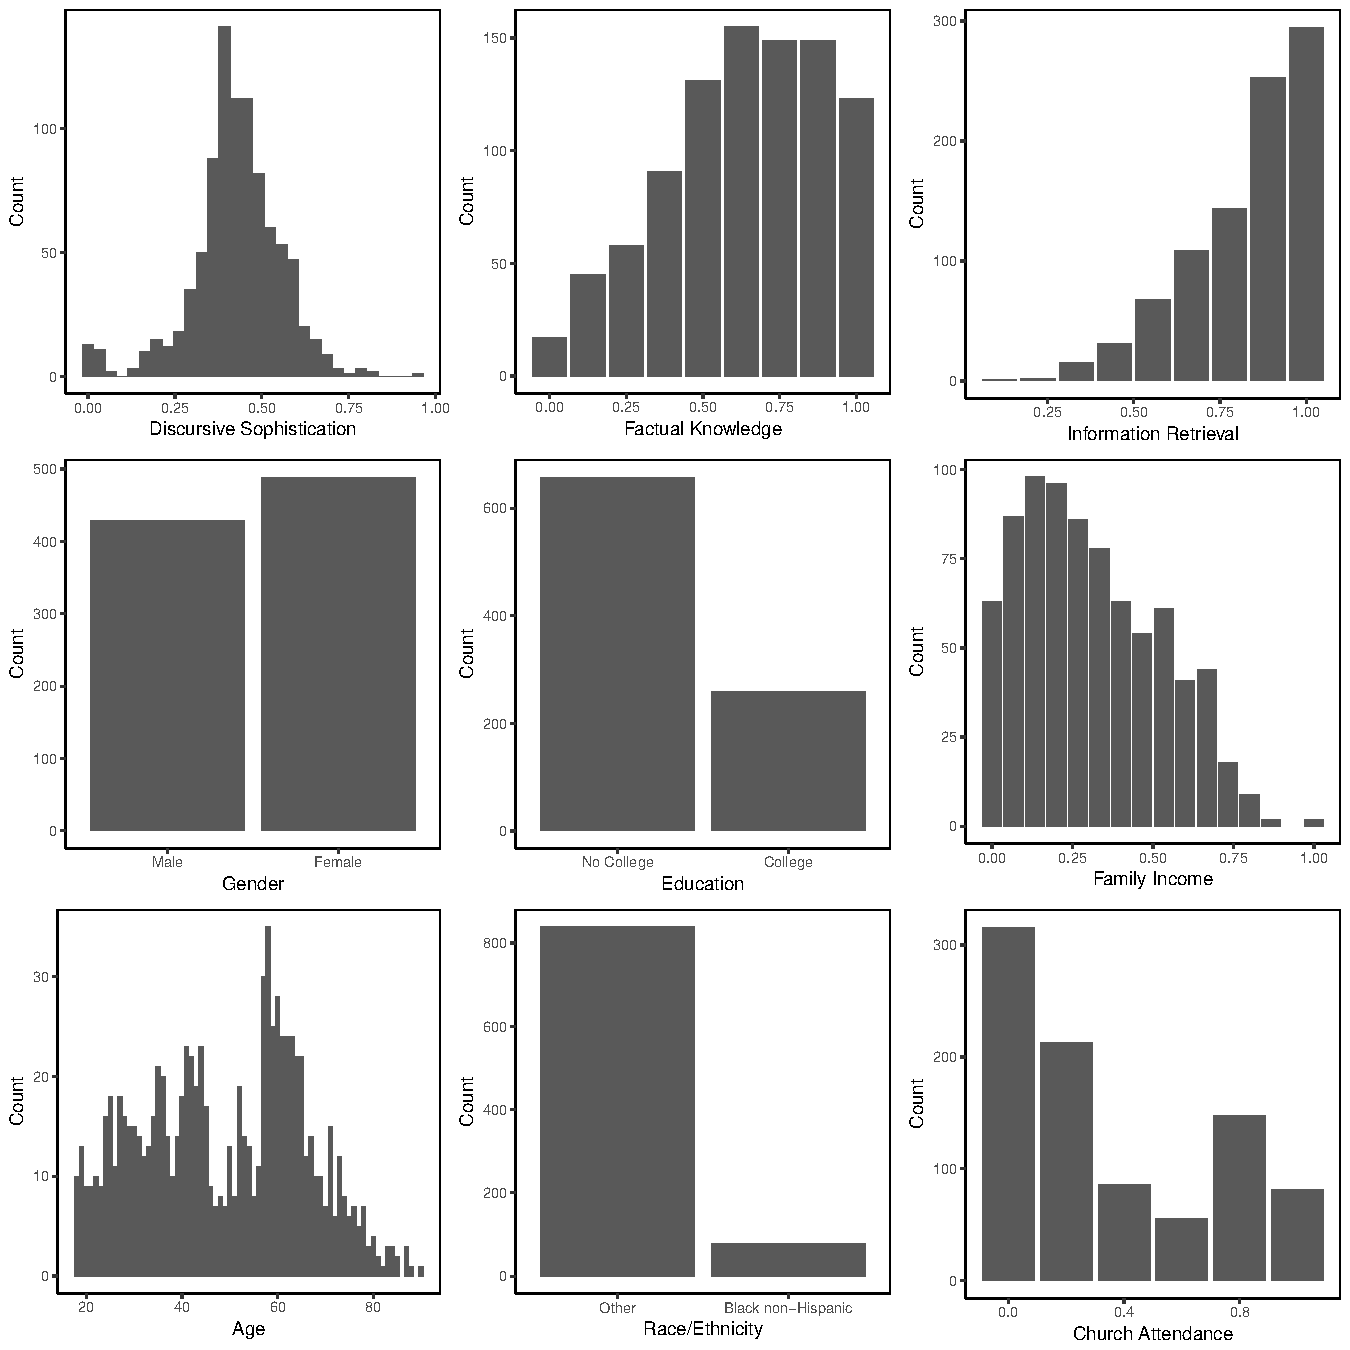
\includegraphics[width=\textwidth]{/data/Dropbox/Uni/projects/2016/knowledge/fig/descriptives_yg.pdf}
\caption[Histogram of variables included in 2015 YouGov survey]{Histogram of variables included in 2015 YouGov survey.}\label{fig:descriptives_yg}
\end{figure}


\clearpage
\section{Robustness Checks}\label{app:personality}
%\renewcommand\thefigure{D.\arabic{figure}}
%\renewcommand\thetable{D.\arabic{table}}
%\setcounter{figure}{0}
%\setcounter{table}{0}

\subsection{Controlling for Personality Characteristics}
\begin{figure}[h]\centering
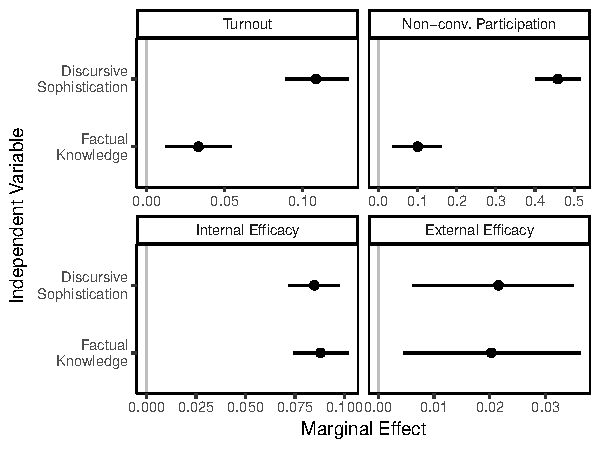
\includegraphics{/data/Dropbox/Uni/projects/2016/knowledge/fig/knoweff_personality.pdf}
\caption[Effects of sophistication on political engagement controlling for personality characteristics in the 2012 and 2016 ANES]{Effects of sophistication on internal efficacy, external efficacy, non-conventional participation, and turnout in the 2012 and 2016 ANES. For each dependent variable, the figure displays the change in expected values after increasing each sophistication measure from -1 to +1 standard deviation from its mean (including 95\% confidence intervals). Model estimates are based on logistic regression (turnout) or OLS (internal efficacy, external efficacy, non-conventional participation). Both sophistication measure are included simultaneously while controlling for gender, education, income, age, race, church attendance, survey mode, Wordsum vocabulary scores, as well as personality characteristics (extraversion and being reserved). Full model results are presented in the appendix, Tables \ref{tab:knoweff2012_personality} and \ref{tab:knoweff2016_personality}.
}\label{fig:knoweff_personality}
\end{figure}

\clearpage
\subsection{Controlling for Individual Response Length}
\begin{figure}[h]\centering
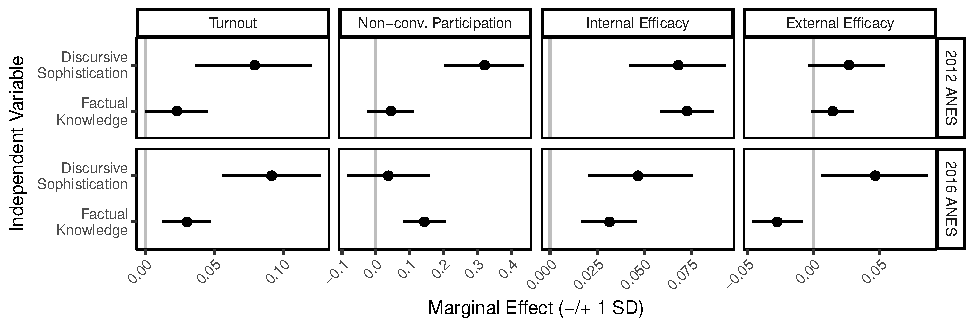
\includegraphics{/data/Dropbox/Uni/projects/2016/knowledge/fig/knoweff_lwc.pdf}
\caption[Effects of sophistication on political engagement controlling for response length in the 2012 and 2016 ANES]{Effects of sophistication on internal efficacy, external efficacy, non-conventional participation, and turnout in the 2012 and 2016 ANES. For each dependent variable, the figure displays the change in expected values after increasing each sophistication measure from -1 to +1 standard deviation from its mean (including 95\% confidence intervals). Model estimates are based on logistic regression (turnout) or OLS (internal efficacy, external efficacy, non-conventional participation). Both sophistication measure are included simultaneously while controlling for gender, education, income, age, race, church attendance, survey mode, Wordsum vocabulary scores, as well as the logged word count across open-ended responses. Full model results are presented in the appendix, Tables \ref{tab:knoweff2012_lwc} and \ref{tab:knoweff2016_lwc}.
}\label{fig:knoweff_lwc}
\end{figure}


\clearpage
\section{Tables of Model Estimates}
%\renewcommand\thefigure{E.\arabic{figure}}
\renewcommand\thetable{E.\arabic{table}}
%\setcounter{figure}{0}
\setcounter{table}{0}

\subsection{Main Analyses}

% Table created by stargazer v.5.2 by Marek Hlavac, Harvard University. E-mail: hlavac at fas.harvard.edu
% Date and time: Thu, Apr 05, 2018 - 12:26:10 AM
% Requires LaTeX packages: dcolumn 
\begin{table}[!htbp] \centering 
  \caption{Effects of sophistication on turnout, non-conventional participation, internal efficacy, 
          and external efficacy in the 2012 ANES. Standard errors in parentheses. Estimates are used for
          Figure 2 in the main text.} 
  \label{tab:knoweff2012} 
\begin{tabular}{@{\extracolsep{0pt}}lD{.}{.}{-3} D{.}{.}{-3} D{.}{.}{-3} D{.}{.}{-3} } 
\\[-1.8ex]\hline 
\hline \\[-1.8ex] 
 & \multicolumn{4}{c}{\textit{Dependent variable:}} \\ 
\cline{2-5} 
 & \multicolumn{1}{c}{Turnout} & \multicolumn{1}{c}{Participation} & \multicolumn{1}{c}{Internal Efficacy} & \multicolumn{1}{c}{External Efficacy} \\ 
\hline \\[-1.8ex] 
 Discursive Soph. & 2.921^{***} & 1.440^{***} & 0.278^{***} & 0.084^{***} \\ 
  & (0.299) & (0.098) & (0.020) & (0.024) \\ 
  Factual Knowledge & 0.432^{*} & 0.099 & 0.158^{***} & 0.032 \\ 
  & (0.218) & (0.075) & (0.016) & (0.018) \\ 
  Female & 0.086 & -0.067^{*} & -0.053^{***} & 0.016^{*} \\ 
  & (0.085) & (0.028) & (0.006) & (0.007) \\ 
  College Degree & 0.350^{**} & 0.159^{***} & 0.022^{**} & 0.035^{***} \\ 
  & (0.112) & (0.034) & (0.007) & (0.008) \\ 
  Family Income & 0.947^{***} & 0.022 & 0.010 & 0.016 \\ 
  & (0.156) & (0.052) & (0.011) & (0.013) \\ 
  Age (log) & 0.988^{***} & 0.102^{**} & -0.006 & -0.014 \\ 
  & (0.105) & (0.038) & (0.008) & (0.009) \\ 
  African American & 0.910^{***} & 0.096^{*} & 0.066^{***} & 0.082^{***} \\ 
  & (0.123) & (0.038) & (0.008) & (0.009) \\ 
  Church Attendance & 0.752^{***} & 0.112^{**} & 0.010 & 0.048^{***} \\ 
  & (0.129) & (0.040) & (0.008) & (0.010) \\ 
  Mode: Online & 0.530^{***} & 0.227^{***} & 0.017^{*} & -0.039^{***} \\ 
  & (0.094) & (0.033) & (0.007) & (0.008) \\ 
  Wordsum Score & 0.638^{**} & 0.403^{***} & 0.092^{***} & 0.013 \\ 
  & (0.219) & (0.076) & (0.016) & (0.019) \\ 
  Constant & -5.019^{***} & -0.598^{***} & 0.326^{***} & 0.352^{***} \\ 
  & (0.401) & (0.145) & (0.030) & (0.035) \\ 
 \hline \\[-1.8ex] 
Observations & \multicolumn{1}{c}{4,716} & \multicolumn{1}{c}{4,692} & \multicolumn{1}{c}{4,996} & \multicolumn{1}{c}{4,985} \\ 
R$^{2}$ &  & \multicolumn{1}{c}{0.124} & \multicolumn{1}{c}{0.161} & \multicolumn{1}{c}{0.043} \\ 
Log Likelihood & \multicolumn{1}{c}{-1,868.199} &  &  &  \\ 
\hline 
\hline \\[-1.8ex] 
\textit{Note:}  & \multicolumn{4}{r}{$^{*}$p$<$0.05; $^{**}$p$<$0.01; $^{***}$p$<$0.001} \\ 
\end{tabular} 
\end{table} 


% Table created by stargazer v.5.2 by Marek Hlavac, Harvard University. E-mail: hlavac at fas.harvard.edu
% Date and time: Tue, Apr 03, 2018 - 12:07:45 AM
% Requires LaTeX packages: dcolumn 
\begin{table}[!htbp] \centering 
  \caption{Effects of sophistication on turnout, non-conventional participation, internal efficacy, 
          and external efficacy in the 2016 ANES. Standard errors in parentheses. Estimates are used for
          Figure 2 in the main text.} 
  \label{tab:knoweff2016} 
\begin{tabular}{@{\extracolsep{0pt}}lD{.}{.}{-3} D{.}{.}{-3} D{.}{.}{-3} D{.}{.}{-3} } 
\\[-1.8ex]\hline 
\hline \\[-1.8ex] 
 & \multicolumn{4}{c}{\textit{Dependent variable:}} \\ 
\cline{2-5} 
 & \multicolumn{1}{c}{Turnout} & \multicolumn{1}{c}{Participation} & \multicolumn{1}{c}{Internal Efficacy} & \multicolumn{1}{c}{External Efficacy} \\ 
\hline \\[-1.8ex] 
 Discursive Soph. & 3.748^{***} & 0.790^{***} & 0.220^{***} & 0.087^{*} \\ 
  & (0.485) & (0.131) & (0.031) & (0.041) \\ 
  Factual Knowledge & 0.733^{***} & 0.271^{***} & 0.059^{***} & -0.052^{**} \\ 
  & (0.219) & (0.058) & (0.014) & (0.018) \\ 
  Female & 0.177 & 0.061^{*} & -0.060^{***} & -0.003 \\ 
  & (0.114) & (0.029) & (0.007) & (0.009) \\ 
  College Degree & 0.556^{***} & 0.091^{**} & 0.058^{***} & 0.056^{***} \\ 
  & (0.141) & (0.033) & (0.008) & (0.010) \\ 
  Family Income & 0.497^{*} & -0.075 & 0.021 & 0.062^{***} \\ 
  & (0.207) & (0.055) & (0.013) & (0.017) \\ 
  Age (log) & 0.837^{***} & -0.111^{**} & 0.020^{*} & -0.005 \\ 
  & (0.139) & (0.038) & (0.009) & (0.012) \\ 
  African American & 1.124^{***} & 0.097 & 0.057^{***} & -0.020 \\ 
  & (0.237) & (0.051) & (0.012) & (0.016) \\ 
  Church Attendance & 1.069^{***} & -0.175^{***} & -0.006 & 0.080^{***} \\ 
  & (0.191) & (0.043) & (0.010) & (0.014) \\ 
  Mode: Online & 0.183 & 0.113^{**} & 0.068^{***} & -0.015 \\ 
  & (0.136) & (0.036) & (0.009) & (0.011) \\ 
  Wordsum Score & 0.934^{***} & 0.399^{***} & 0.103^{***} & 0.015 \\ 
  & (0.275) & (0.079) & (0.019) & (0.025) \\ 
  Constant & -4.235^{***} & 0.213 & 0.233^{***} & 0.336^{***} \\ 
  & (0.534) & (0.151) & (0.036) & (0.048) \\ 
 \hline \\[-1.8ex] 
Observations & \multicolumn{1}{c}{3,487} & \multicolumn{1}{c}{3,040} & \multicolumn{1}{c}{3,038} & \multicolumn{1}{c}{3,039} \\ 
R$^{2}$ &  & \multicolumn{1}{c}{0.062} & \multicolumn{1}{c}{0.147} & \multicolumn{1}{c}{0.043} \\ 
Log Likelihood & \multicolumn{1}{c}{-1,087.769} &  &  &  \\ 
\hline 
\hline \\[-1.8ex] 
\textit{Note:}  & \multicolumn{4}{r}{$^{*}$p$<$0.05; $^{**}$p$<$0.01; $^{***}$p$<$0.001} \\ 
\end{tabular} 
\end{table} 


% Table created by stargazer v.5.2.3 by Marek Hlavac, Social Policy Institute. E-mail: marek.hlavac at gmail.com
% Date and time: Mon, Aug 15, 2022 - 10:21:41 PM
% Requires LaTeX packages: dcolumn 
\begin{table}[!htbp] \centering 
  \caption{Linear regressions predicting information retrieval in the 2015 YouGov study.
          Standard errors in parentheses. Estimates are used for Figure \ref{fig:yg_disease}
          in the main text.} 
  \label{tab:yg_disease} 
\footnotesize 
\begin{tabular}{@{\extracolsep{-25pt}}lD{.}{.}{-3} D{.}{.}{-3} D{.}{.}{-3} } 
\\[-1.8ex]\hline 
\hline \\[-1.8ex] 
 & \multicolumn{3}{c}{\textit{Dependent variable:}} \\ 
\cline{2-4} 
 & \multicolumn{3}{c}{Information Retrieval} \\ 
\\[-1.8ex] & \multicolumn{1}{c}{(1)} & \multicolumn{1}{c}{(2)} & \multicolumn{1}{c}{(3)}\\ 
\hline \\[-1.8ex] 
 Discursive Soph. & 0.039^{***} & 0.033^{***} & 0.032^{***} \\ 
  & (0.006) & (0.006) & (0.006) \\ 
  Factual Knowledge & 0.030^{***} & 0.035^{***} & 0.034^{***} \\ 
  & (0.006) & (0.007) & (0.007) \\ 
  Disc. X Factual &  &  & -0.008 \\ 
  &  &  & (0.006) \\ 
  Female &  & 0.043^{***} & 0.043^{***} \\ 
  &  & (0.012) & (0.012) \\ 
  Age &  & 0.001^{*} & 0.001^{*} \\ 
  &  & (0.0004) & (0.0004) \\ 
  Black &  & -0.027 & -0.026 \\ 
  &  & (0.021) & (0.021) \\ 
  College Degree &  & 0.017 & 0.017 \\ 
  &  & (0.014) & (0.014) \\ 
  Household Income &  & -0.061^{*} & -0.060^{*} \\ 
  &  & (0.030) & (0.030) \\ 
  Church Attendance &  & -0.059^{***} & -0.059^{***} \\ 
  &  & (0.017) & (0.017) \\ 
  Constant & 0.828^{***} & 0.807^{***} & 0.811^{***} \\ 
  & (0.005) & (0.021) & (0.021) \\ 
 \hline \\[-1.8ex] 
Observations & \multicolumn{1}{c}{918} & \multicolumn{1}{c}{792} & \multicolumn{1}{c}{792} \\ 
R$^{2}$ & \multicolumn{1}{c}{0.100} & \multicolumn{1}{c}{0.137} & \multicolumn{1}{c}{0.139} \\ 
\hline 
\hline \\[-1.8ex] 
\textit{Note:}  & \multicolumn{3}{r}{$^{*}$p$<$0.05; $^{**}$p$<$0.01; $^{***}$p$<$0.001} \\ 
\end{tabular} 
\end{table} 


% Table created by stargazer v.5.2 by Marek Hlavac, Harvard University. E-mail: hlavac at fas.harvard.edu
% Date and time: Mon, Apr 02, 2018 - 03:43:21 PM
% Requires LaTeX packages: dcolumn 
\begin{table}[!htbp] \centering 
  \caption{Effects of gender on discursive sophistication and factual knowledge in the 
          2012 ANES and 2016 ANES. Standard errors in parentheses. Estimates are used for 
          Figure 8 in the main text.} 
  \label{tab:determinants_anes} 
\begin{tabular}{@{\extracolsep{0pt}}lD{.}{.}{-3} D{.}{.}{-3} D{.}{.}{-3} D{.}{.}{-3} } 
\\[-1.8ex]\hline 
\hline \\[-1.8ex] 
 & \multicolumn{4}{c}{\textit{Dependent variable:}} \\ 
\cline{2-5} 
\\[-1.8ex] & \multicolumn{2}{c}{Discursive Sophistication} & \multicolumn{2}{c}{Factual Knowledge} \\ 
 & \multicolumn{1}{c}{2012 ANES} & \multicolumn{1}{c}{2016 ANES} & \multicolumn{1}{c}{2012 ANES} & \multicolumn{1}{c}{2016 ANES} \\ 
\hline \\[-1.8ex] 
 Female & 0.003 & -0.003 & -0.050^{***} & -0.031^{**} \\ 
  & (0.004) & (0.004) & (0.006) & (0.010) \\ 
  Media Exposure & 0.042^{***} & 0.046^{***} & 0.067^{***} & 0.075^{***} \\ 
  & (0.010) & (0.009) & (0.014) & (0.021) \\ 
  Discussion Freqency & 0.119^{***} & 0.040^{***} & 0.062^{***} & 0.061^{***} \\ 
  & (0.007) & (0.007) & (0.010) & (0.015) \\ 
  College Degree & 0.070^{***} & 0.046^{***} & 0.091^{***} & 0.047^{***} \\ 
  & (0.005) & (0.005) & (0.007) & (0.010) \\ 
  Family Income & 0.052^{***} & 0.033^{***} & 0.116^{***} & 0.088^{***} \\ 
  & (0.008) & (0.008) & (0.010) & (0.018) \\ 
  Age (log) & 0.017^{**} & -0.002 & 0.081^{***} & 0.091^{***} \\ 
  & (0.006) & (0.006) & (0.008) & (0.014) \\ 
  African American & -0.005 & -0.034^{***} & -0.085^{***} & -0.004 \\ 
  & (0.005) & (0.008) & (0.008) & (0.017) \\ 
  Church Attendance & 0.004 & 0.004 & -0.003 & -0.017 \\ 
  & (0.006) & (0.006) & (0.008) & (0.014) \\ 
  Mode: Online & -0.045^{***} & -0.122^{***} & 0.092^{***} & 0.086^{***} \\ 
  & (0.005) & (0.005) & (0.006) & (0.011) \\ 
  Constant & 0.192^{***} & 0.323^{***} & 0.195^{***} & 0.016 \\ 
  & (0.021) & (0.022) & (0.030) & (0.051) \\ 
 \hline \\[-1.8ex] 
Observations & \multicolumn{1}{c}{4,690} & \multicolumn{1}{c}{2,611} & \multicolumn{1}{c}{4,690} & \multicolumn{1}{c}{2,602} \\ 
R$^{2}$ & \multicolumn{1}{c}{0.178} & \multicolumn{1}{c}{0.270} & \multicolumn{1}{c}{0.282} & \multicolumn{1}{c}{0.106} \\ 
\hline 
\hline \\[-1.8ex] 
\textit{Note:}  & \multicolumn{4}{r}{$^{*}$p$<$0.05; $^{**}$p$<$0.01; $^{***}$p$<$0.001} \\ 
\end{tabular} 
\end{table} 


% Table created by stargazer v.5.2 by Marek Hlavac, Harvard University. E-mail: hlavac at fas.harvard.edu
% Date and time: Mon, Apr 02, 2018 - 07:34:30 PM
% Requires LaTeX packages: dcolumn 
\begin{table}[!htbp] \centering 
  \caption{Effects of gender on discursive sophistication and factual knowledge in the 
          2015 YouGov Study. Standard errors in parentheses. Estimates are used for 
          Figure 8 in the main text.} 
  \label{tab:determinants_yg} 
\begin{tabular}{@{\extracolsep{0pt}}lD{.}{.}{-3} D{.}{.}{-3} } 
\\[-1.8ex]\hline 
\hline \\[-1.8ex] 
 & \multicolumn{2}{c}{\textit{Dependent variable:}} \\ 
\cline{2-3} 
 & \multicolumn{1}{c}{Discursive Sophistication} & \multicolumn{1}{c}{Factual Knowledge} \\ 
\hline \\[-1.8ex] 
 Female & 0.011 & -0.157^{***} \\ 
  & (0.009) & (0.016) \\ 
  College Degree & 0.030^{**} & 0.108^{***} \\ 
  & (0.011) & (0.019) \\ 
  Family Income & -0.017 & 0.233^{***} \\ 
  & (0.023) & (0.041) \\ 
  Age (log) & 0.044^{***} & 0.135^{***} \\ 
  & (0.012) & (0.021) \\ 
  African American & -0.063^{***} & -0.086^{**} \\ 
  & (0.017) & (0.029) \\ 
  Church Attendance & -0.006 & -0.051^{*} \\ 
  & (0.013) & (0.023) \\ 
  Constant & 0.258^{***} & 0.125 \\ 
  & (0.047) & (0.083) \\ 
 \hline \\[-1.8ex] 
Observations & \multicolumn{1}{c}{792} & \multicolumn{1}{c}{792} \\ 
R$^{2}$ & \multicolumn{1}{c}{0.048} & \multicolumn{1}{c}{0.272} \\ 
\hline 
\hline \\[-1.8ex] 
\textit{Note:}  & \multicolumn{2}{r}{$^{*}$p$<$0.05; $^{**}$p$<$0.01; $^{***}$p$<$0.001} \\ 
\end{tabular} 
\end{table} 


\clearpage
\subsection{Robustness Checks}

% Table created by stargazer v.5.2 by Marek Hlavac, Harvard University. E-mail: hlavac at fas.harvard.edu
% Date and time: Mon, Apr 02, 2018 - 03:53:40 PM
% Requires LaTeX packages: dcolumn 
\begin{table}[!htbp] \centering 
  \caption{Effects of sophistication on turnout, non-conventional participation, internal efficacy, 
          and external efficacy controlling for personality characteristics in the 2012 ANES. 
          Standard errors in parentheses. Estimates are used for Figure \ref{fig:knoweff_personality} 
          in the appendix.} 
  \label{tab:knoweff2012_personality} 
\begin{tabular}{@{\extracolsep{0pt}}lD{.}{.}{-3} D{.}{.}{-3} D{.}{.}{-3} D{.}{.}{-3} } 
\\[-1.8ex]\hline 
\hline \\[-1.8ex] 
 & \multicolumn{4}{c}{\textit{Dependent variable:}} \\ 
\cline{2-5} 
 & \multicolumn{1}{c}{Turnout} & \multicolumn{1}{c}{Participation} & \multicolumn{1}{c}{Internal Efficacy} & \multicolumn{1}{c}{External Efficacy} \\ 
\hline \\[-1.8ex] 
 Discursive Soph. & 2.967^{***} & 1.432^{***} & 0.275^{***} & 0.095^{***} \\ 
  & (0.305) & (0.100) & (0.021) & (0.025) \\ 
  Factual Knowledge & 0.441^{*} & 0.105 & 0.165^{***} & 0.035 \\ 
  & (0.218) & (0.075) & (0.016) & (0.019) \\ 
  Female & 0.085 & -0.080^{**} & -0.060^{***} & 0.009 \\ 
  & (0.085) & (0.028) & (0.006) & (0.007) \\ 
  College Degree & 0.350^{**} & 0.160^{***} & 0.020^{**} & 0.032^{***} \\ 
  & (0.112) & (0.034) & (0.007) & (0.008) \\ 
  Family Income & 0.946^{***} & -0.0001 & 0.006 & 0.010 \\ 
  & (0.157) & (0.052) & (0.011) & (0.013) \\ 
  Age (log) & 0.981^{***} & 0.102^{**} & -0.003 & -0.017 \\ 
  & (0.106) & (0.039) & (0.008) & (0.010) \\ 
  African American & 0.893^{***} & 0.093^{*} & 0.066^{***} & 0.077^{***} \\ 
  & (0.124) & (0.038) & (0.008) & (0.010) \\ 
  Church Attendance & 0.728^{***} & 0.103^{**} & 0.006 & 0.044^{***} \\ 
  & (0.130) & (0.040) & (0.008) & (0.010) \\ 
  Mode: Online & 0.544^{***} & 0.251^{***} & 0.022^{**} & -0.032^{***} \\ 
  & (0.096) & (0.033) & (0.007) & (0.008) \\ 
  Wordsum Score & 0.643^{**} & 0.409^{***} & 0.092^{***} & 0.020 \\ 
  & (0.220) & (0.076) & (0.016) & (0.019) \\ 
  Extraversion & 0.031 & 0.033^{***} & 0.009^{***} & 0.020^{***} \\ 
  & (0.030) & (0.010) & (0.002) & (0.002) \\ 
  Reserved & 0.009 & -0.023^{**} & -0.005^{**} & 0.002 \\ 
  & (0.026) & (0.009) & (0.002) & (0.002) \\ 
  Constant & -5.185^{***} & -0.638^{***} & 0.297^{***} & 0.254^{***} \\ 
  & (0.450) & (0.158) & (0.034) & (0.039) \\ 
 \hline \\[-1.8ex] 
Observations & \multicolumn{1}{c}{4,691} & \multicolumn{1}{c}{4,685} & \multicolumn{1}{c}{4,691} & \multicolumn{1}{c}{4,679} \\ 
R$^{2}$ &  & \multicolumn{1}{c}{0.128} & \multicolumn{1}{c}{0.171} & \multicolumn{1}{c}{0.059} \\ 
Log Likelihood & \multicolumn{1}{c}{-1,861.487} &  &  &  \\ 
\hline 
\hline \\[-1.8ex] 
\textit{Note:}  & \multicolumn{4}{r}{$^{*}$p$<$0.05; $^{**}$p$<$0.01; $^{***}$p$<$0.001} \\ 
\end{tabular} 
\end{table} 


% Table created by stargazer v.5.2 by Marek Hlavac, Harvard University. E-mail: hlavac at fas.harvard.edu
% Date and time: Thu, Apr 05, 2018 - 07:38:52 AM
% Requires LaTeX packages: dcolumn 
\begin{table}[!htbp] \centering 
  \caption{Effects of sophistication on turnout, non-conventional participation, internal efficacy, 
          and external efficacy controlling for personality characteristics in the 2016 ANES. 
          Standard errors in parentheses. Estimates are used for Figure \ref{fig:knoweff_personality} 
          in the appendix.} 
  \label{tab:knoweff2016_personality} 
\begin{tabular}{@{\extracolsep{0pt}}lD{.}{.}{-3} D{.}{.}{-3} D{.}{.}{-3} D{.}{.}{-3} } 
\\[-1.8ex]\hline 
\hline \\[-1.8ex] 
 & \multicolumn{4}{c}{\textit{Dependent variable:}} \\ 
\cline{2-5} 
 & \multicolumn{1}{c}{Turnout} & \multicolumn{1}{c}{Participation} & \multicolumn{1}{c}{Internal Efficacy} & \multicolumn{1}{c}{External Efficacy} \\ 
\hline \\[-1.8ex] 
 Discursive Soph. & 3.936^{***} & 0.760^{***} & 0.213^{***} & 0.070 \\ 
  & (0.543) & (0.132) & (0.031) & (0.042) \\ 
  Factual Knowledge & 0.717^{**} & 0.260^{***} & 0.056^{***} & -0.052^{**} \\ 
  & (0.241) & (0.059) & (0.014) & (0.019) \\ 
  Female & 0.172 & 0.046 & -0.064^{***} & -0.004 \\ 
  & (0.125) & (0.029) & (0.007) & (0.009) \\ 
  College Degree & 0.616^{***} & 0.085^{**} & 0.056^{***} & 0.055^{***} \\ 
  & (0.155) & (0.033) & (0.008) & (0.010) \\ 
  Family Income & 0.471^{*} & -0.085 & 0.017 & 0.060^{***} \\ 
  & (0.230) & (0.055) & (0.013) & (0.017) \\ 
  Age (log) & 0.894^{***} & -0.119^{**} & 0.018^{*} & -0.010 \\ 
  & (0.153) & (0.039) & (0.009) & (0.012) \\ 
  African American & 1.228^{***} & 0.102^{*} & 0.057^{***} & -0.026 \\ 
  & (0.267) & (0.052) & (0.012) & (0.016) \\ 
  Church Attendance & 0.930^{***} & -0.172^{***} & -0.007 & 0.078^{***} \\ 
  & (0.205) & (0.043) & (0.010) & (0.014) \\ 
  Mode: Online & 0.199 & 0.111^{**} & 0.069^{***} & -0.015 \\ 
  & (0.148) & (0.036) & (0.009) & (0.011) \\ 
  Wordsum Score & 0.999^{**} & 0.436^{***} & 0.114^{***} & 0.022 \\ 
  & (0.311) & (0.080) & (0.019) & (0.025) \\ 
  Extraversion & 0.090^{*} & 0.023^{*} & 0.011^{***} & 0.012^{***} \\ 
  & (0.041) & (0.010) & (0.002) & (0.003) \\ 
  Reserved & 0.005 & -0.013 & -0.002 & 0.005 \\ 
  & (0.037) & (0.009) & (0.002) & (0.003) \\ 
  Constant & -4.948^{***} & 0.196 & 0.199^{***} & 0.277^{***} \\ 
  & (0.646) & (0.163) & (0.039) & (0.051) \\ 
 \hline \\[-1.8ex] 
Observations & \multicolumn{1}{c}{2,999} & \multicolumn{1}{c}{3,011} & \multicolumn{1}{c}{3,012} & \multicolumn{1}{c}{3,012} \\ 
R$^{2}$ &  & \multicolumn{1}{c}{0.065} & \multicolumn{1}{c}{0.155} & \multicolumn{1}{c}{0.047} \\ 
Log Likelihood & \multicolumn{1}{c}{-907.430} &  &  &  \\ 
\hline 
\hline \\[-1.8ex] 
\textit{Note:}  & \multicolumn{4}{r}{$^{*}$p$<$0.05; $^{**}$p$<$0.01; $^{***}$p$<$0.001} \\ 
\end{tabular} 
\end{table} 


% Table created by stargazer v.5.2 by Marek Hlavac, Harvard University. E-mail: hlavac at fas.harvard.edu
% Date and time: Thu, Apr 19, 2018 - 11:39:47 PM
% Requires LaTeX packages: dcolumn 
\begin{table}[!htbp] \centering 
  \caption{Effects of sophistication on turnout, non-conventional participation, internal efficacy, 
          and external efficacy controlling for individual response length in the 2012 ANES. 
          Standard errors in parentheses. Estimates are used for Figure \ref{fig:knoweff_lwc} 
          in the appendix.} 
  \label{tab:knoweff2012_lwc} 
\begin{tabular}{@{\extracolsep{0pt}}lD{.}{.}{-3} D{.}{.}{-3} D{.}{.}{-3} D{.}{.}{-3} } 
\\[-1.8ex]\hline 
\hline \\[-1.8ex] 
 & \multicolumn{4}{c}{\textit{Dependent variable:}} \\ 
\cline{2-5} 
 & \multicolumn{1}{c}{Turnout} & \multicolumn{1}{c}{Participation} & \multicolumn{1}{c}{Internal Efficacy} & \multicolumn{1}{c}{External Efficacy} \\ 
\hline \\[-1.8ex] 
 Discursive Soph. & 2.053 & 0.967 & 0.215 & 0.082 \\ 
  & (0.543) & (0.186) & (0.039) & (0.045) \\ 
  Factual Knowledge & 0.426 & 0.096 & 0.158 & 0.032 \\ 
  & (0.218) & (0.075) & (0.016) & (0.018) \\ 
  Female & 0.067 & -0.076 & -0.054 & 0.016 \\ 
  & (0.085) & (0.028) & (0.006) & (0.007) \\ 
  College Degree & 0.370 & 0.167 & 0.023 & 0.035 \\ 
  & (0.113) & (0.034) & (0.007) & (0.008) \\ 
  Family Income & 0.948 & 0.026 & 0.011 & 0.016 \\ 
  & (0.156) & (0.052) & (0.011) & (0.013) \\ 
  Age (log) & 0.976 & 0.094 & -0.007 & -0.014 \\ 
  & (0.106) & (0.039) & (0.008) & (0.009) \\ 
  African American & 0.896 & 0.088 & 0.064 & 0.082 \\ 
  & (0.123) & (0.038) & (0.008) & (0.009) \\ 
  Church Attendance & 0.758 & 0.113 & 0.010 & 0.048 \\ 
  & (0.129) & (0.040) & (0.008) & (0.010) \\ 
  Mode: Online & 0.574 & 0.246 & 0.020 & -0.039 \\ 
  & (0.097) & (0.034) & (0.007) & (0.008) \\ 
  Wordsum Score & 0.626 & 0.396 & 0.091 & 0.013 \\ 
  & (0.219) & (0.076) & (0.016) & (0.019) \\ 
  Word Count (log) & 0.970 & 0.539 & 0.071 & 0.003 \\ 
  & (0.507) & (0.180) & (0.037) & (0.044) \\ 
  Constant & -5.237 & -0.710 & 0.311 & 0.352 \\ 
  & (0.418) & (0.150) & (0.031) & (0.036) \\ 
 \hline \\[-1.8ex] 
Observations & \multicolumn{1}{c}{4,716} & \multicolumn{1}{c}{4,692} & \multicolumn{1}{c}{4,996} & \multicolumn{1}{c}{4,985} \\ 
R$^{2}$ &  & \multicolumn{1}{c}{0.126} & \multicolumn{1}{c}{0.162} & \multicolumn{1}{c}{0.043} \\ 
Log Likelihood & \multicolumn{1}{c}{-1,866.366} &  &  &  \\ 
\hline 
\hline \\[-1.8ex] 
\end{tabular} 
\end{table} 


% Table created by stargazer v.5.2 by Marek Hlavac, Harvard University. E-mail: hlavac at fas.harvard.edu
% Date and time: Mon, Apr 02, 2018 - 12:18:45 PM
% Requires LaTeX packages: dcolumn 
\begin{table}[!htbp] \centering 
  \caption{Effects of sophistication on turnout, non-conventional participation, internal efficacy, 
          and external efficacy controlling for individual response length in the 2016 ANES. 
          Standard errors in parentheses. Estimates are used for Figure \ref{fig:knoweff_lwc} 
          in the appendix.} 
  \label{tab:knoweff2016_lwc} 
\begin{tabular}{@{\extracolsep{0pt}}lD{.}{.}{-3} D{.}{.}{-3} D{.}{.}{-3} D{.}{.}{-3} } 
\\[-1.8ex]\hline 
\hline \\[-1.8ex] 
 & \multicolumn{4}{c}{\textit{Dependent variable:}} \\ 
\cline{2-5} 
 & \multicolumn{1}{c}{Turnout} & \multicolumn{1}{c}{Participation} & \multicolumn{1}{c}{Internal Efficacy} & \multicolumn{1}{c}{External Efficacy} \\ 
\hline \\[-1.8ex] 
 Discursive Soph. & 4.519^{***} & 0.154 & 0.183^{**} & 0.178^{*} \\ 
  & (0.855) & (0.236) & (0.056) & (0.075) \\ 
  Factual Knowledge & 0.734^{***} & 0.272^{***} & 0.059^{***} & -0.052^{**} \\ 
  & (0.219) & (0.058) & (0.014) & (0.018) \\ 
  Female & 0.187 & 0.053 & -0.060^{***} & -0.002 \\ 
  & (0.114) & (0.029) & (0.007) & (0.009) \\ 
  College Degree & 0.551^{***} & 0.098^{**} & 0.059^{***} & 0.055^{***} \\ 
  & (0.141) & (0.033) & (0.008) & (0.010) \\ 
  Family Income & 0.497^{*} & -0.072 & 0.021 & 0.062^{***} \\ 
  & (0.207) & (0.054) & (0.013) & (0.017) \\ 
  Age (log) & 0.835^{***} & -0.111^{**} & 0.020^{*} & -0.005 \\ 
  & (0.139) & (0.038) & (0.009) & (0.012) \\ 
  African American & 1.125^{***} & 0.089 & 0.056^{***} & -0.019 \\ 
  & (0.237) & (0.051) & (0.012) & (0.016) \\ 
  Church Attendance & 1.065^{***} & -0.171^{***} & -0.006 & 0.080^{***} \\ 
  & (0.191) & (0.043) & (0.010) & (0.014) \\ 
  Mode: Online & 0.105 & 0.183^{***} & 0.071^{***} & -0.026^{*} \\ 
  & (0.161) & (0.043) & (0.010) & (0.013) \\ 
  Wordsum Score & 0.930^{***} & 0.403^{***} & 0.104^{***} & 0.016 \\ 
  & (0.275) & (0.079) & (0.019) & (0.025) \\ 
  Word Count (log) & -0.854 & 0.707^{**} & 0.035 & -0.110 \\ 
  & (0.815) & (0.226) & (0.054) & (0.072) \\ 
  Constant & -3.978^{***} & 0.008 & 0.225^{***} & 0.371^{***} \\ 
  & (0.588) & (0.166) & (0.040) & (0.052) \\ 
 \hline \\[-1.8ex] 
Observations & \multicolumn{1}{c}{3,487} & \multicolumn{1}{c}{3,040} & \multicolumn{1}{c}{3,038} & \multicolumn{1}{c}{3,039} \\ 
R$^{2}$ &  & \multicolumn{1}{c}{0.065} & \multicolumn{1}{c}{0.146} & \multicolumn{1}{c}{0.043} \\ 
Log Likelihood & \multicolumn{1}{c}{-1,086.955} &  &  &  \\ 
\hline 
\hline \\[-1.8ex] 
\textit{Note:}  & \multicolumn{4}{r}{$^{*}$p$<$0.05; $^{**}$p$<$0.01; $^{***}$p$<$0.001} \\ 
\end{tabular} 
\end{table} 






\end{document}